\documentclass[final,12pt,3p,times,authoryear]{elsarticle}
\newif\ifANONYMOUS\ANONYMOUStrue
\newif\iffrontonly\frontonlyfalse
%%% RENOVE THE FOLLOWING LINE TO REMOVE THE AUTHOR NAMES AUTHOR REFERENCES
\ANONYMOUSfalse
%%%%%%%%%%%%%%%%%%%%

\usepackage[dvipsnames,svgnames,x11names]{xcolor}
\usepackage{array}

\newcommand\cmr[1]{{\fontfamily{cmr}\selectfont#1}}

\newcommand\maybecolor[1]{#1}
\let\maybecolor=\color % Comment this out to remove author marks.
                       % \TODO needs to be removed by hand.



\newcommand{\eg}[1]{{\it e.g.\spacefactor1000\relax#1}}
\newcommand{\ie}[1]{{\it i.e.\spacefactor1000\relax#1}}
\renewcommand{\ie}[1]{that is,}
\renewcommand{\eg}[1]{for example,}

\usepackage[explicit]{titlesec}
\setcounter{secnumdepth}{2}
\titleformat{\section}[runin]{\bf}{\thesection}{1em}{\sc #1 }
\titleformat{\subsection}[runin]{\bf}{\thesubsection}{1em}{\sc #1 }
\titleformat{\subsubsection}[runin]{\bf}{\thesubsubsection}{1em}{\sc #1 \hspace{1em}}


\ifx\doiresolver\undefined\def\doiresolver{http://dx.doi.org/}\fi
\ifx\texorpdfstring\undefined\newcommand\texorpdfstring[2]{#1}\fi

%\def\doiresolver{}

\usepackage{natbib}
\usepackage{graphicx}
\usepackage{amsmath}
\usepackage{amssymb}
%\usepackage{multirow}
\usepackage{longtable}
\usepackage{tipa}
\usepackage{float}
%\usepackage{subfigure}
\newcommand{\TODO}[1]{\begingroup\color{red}#1\endgroup}
\newcommand{\LM}[1]{\begingroup\maybecolor{magenta}#1\endgroup}
\newcommand{\PFS}[1]{\begingroup\maybecolor{green}#1\endgroup}
\newcommand{\NOTE}[1]{\begingroup\maybecolor{blue}#1\endgroup}
\newcommand{\NR}[1]{\begingroup\maybecolor{Orange}#1\endgroup}
\newcommand{\DB}[1]{\begingroup\maybecolor{Cerulean}#1\endgroup}
\newcommand{\HY}[1]{\begingroup\maybecolor{OliveGreen}#1\endgroup}
\newcommand{\TB}[1]{\begingroup\maybecolor{Fuchsia}#1\endgroup}
\definecolor{pinegreen}{rgb}{0.0,0.47,0.44}
\newcommand{\NEW}[1]{\begingroup\color{pinegreen}#1\endgroup} 
%TB
%mark ups for language style
\newcommand{\LING}[1]{\textit{#1}}
\newcommand{\TT}[1]{\textsc{#1}}
\newcommand{\QUOTE}[1]{`#1'}
 
\usepackage{endnotes}
\def\notesname{}

 
\renewcommand{\cite}{\citep}
\renewcommand{\floatpagefraction}{.9999}
\renewcommand{\textfraction}{.0001}
\renewcommand{\dblfloatpagefraction}{.999}
\renewcommand{\dbltopfraction}{0.999}
\renewcommand{\bottomfraction}{0.999}
\makeatletter
\def\paragraph{\secdef{\els@aparagraph}{\els@bparagraph}}
\def\els@aparagraph[#1]#2{\elsparagraph[#1]{#2}}
\def\els@bparagraph#1{\elsparagraph*{#1}}
\makeatother

\usepackage{setspace}

\newcommand{\othercall}[2]{{\escapechar-1\relax
                      \edef\temp{\expandafter\string\csname#2\endcsname}%
                      \expandafter}\expandafter#1\expandafter{\temp}}
\newcommand{\doemail}[1]{\href{mailto:#1}{\tt #1}}
\newcommand{\email}[1]{\othercall\doemail{#1}}

% Pretty up doi and url
{\catcode`\!=\catcode`\%
  \gdef\activateurlcodes{\catcode`\/=\active
                        \catcode`\-=\active
                        \catcode`\(=\active
                        \catcode`\)=\active
                        \catcode`\.=\active
                        \catcode`\&=\active
                        \catcode`\_=\active
                        \catcode`\^=\active
                        \catcode`\$=\active
                        \catcode`\#=\active
                        \catcode`\%=\active
                        \catcode`\:=\active}
 \activateurlcodes
 \gdef\deactivateurlcodes{\def/{\string/}!
                          \def-{\string-}!
                          \def({\string(}!
                          \def){\string)}!
                          \def.{\string.}!
                          \def&{\string&}!
                          \def_{\string_}!
                          \def^{\string^}!
                          \def${\string$}!
                          \def#{\string#}!
                          \def%{\string%}!
                          \def:{\string:}}
 \gdef/{\string/\discretionary{}{}{}}
 \gdef-{\string-\discretionary{}{}{}}
 \gdef({\discretionary{}{}{}\string(}
 \gdef){\string)\discretionary{}{}{}}
 \gdef.{\string.\discretionary{}{}{}}
 \gdef&{\string&\discretionary{}{}{}}
 \gdef_{\_\discretionary{}{}{}}
 \gdef^{\string^}
 \gdef${\string$}
 \gdef#{\string#}
 \gdef%{\string%}
 \gdef:{\string:\discretionary{}{}{}}
}
%\expandafter\ifx\csname url\endcsname\relax
\def\url#1{{\deactivateurlcodes\edef\tmp{\noexpand\href{#1}}%
            \expandafter}\tmp{\texttt #1}}
%\fi
\let\origurl=\url
\def\url{{\activateurlcodes\expandafter}\origurl}
\def\email#1{{\deactivateurlcodes\edef\tmp{\noexpand\href{mailto:#1}}%
    \expandafter}\tmp{\texttt #1}}
\let\origemail=\email
\def\email{{\activateurlcodes\expandafter}\origemail}
\expandafter\ifx\csname doi\endcsname\relax
\def\doi#1{{\deactivateurlcodes\edef\tmp{\noexpand\href{\doiresolver#1}}%
            \expandafter}\tmp{\texttt doi:#1}}\fi
\let\origdoi=\doi
\def\doi{{\activateurlcodes\expandafter}\origdoi}

\newcommand\blfootnote[1]{%
  \begingroup
  \renewcommand\thefootnote{}\footnote{#1}%
  \addtocounter{footnote}{-1}%
  \endgroup
}

\journal{Preprint}

\usepackage{hyperref}

%page numbering in top right corner
\usepackage{fancyhdr}
\pagestyle{fancy}
\fancyhf{}
\fancyhead[R]{\thepage}

\begin{document}
\begin{frontmatter}


\ifANONYMOUS
\author{}
\else
\author[SFI,LANL]{Tanmoy Bhattacharya\corref{cor}}
\author[ZURI,SHH]{Dami\'{a}n E. Blasi}
\author[UNM]{William Croft}
\author[Marburg]{Michael Cysouw}
\author[ASU]{Daniel Hruschka}
\author[UNM]{Ian Maddieson}
\author[Leipzig]{Lydia M{\"u}ller}
\author[Leipzig,MIS]{Nancy Retzlaff}
\author[SFI,GMU,RI]{Eric Smith}
\author[SFI,MPI,Leipzig]{Peter F. Stadler\corref{cor}}
\author[Moscow]{George Starostin}
\author[SFI,Oxford]{Hyejin Youn}
\address[SFI]{Santa Fe Institute, 1399 Hyde Park Rd., Santa Fe, NM
             87501, USA}
\address[LANL]{Theoretical Division, Los Alamos National Laboratory,
             Los Alamos, NM 87545-0285, USA}
\address[MIS]{Max Planck Institute for Mathematics in the Sciences,
            D-04103 Leipzig, Germany}
\address[ZURI]{University of Z\"{u}rich,
            Z\"{u}rich, Switzerland}
\address[SHH]{Max Planck Institute for the Science of Human History,
            Jena, Germany}
\address[EVA]{Max Planck Institute for Evolutionary Anthropology,
            D-04103 Leipzig, Germany}
\address[UNM]{Linguistics, University of New Mexico, Albuquerque,
             NM 87131-0001, USA}
\address[Marburg]{Forschungszentrum Deutscher Sprachatlas, Philipps
                 Universit\"at Marburg, Marburg, Germany}
\address[ASU]{School of Human Evolution and Social Change, Arizona State 
            University, Tempe AZ 85287, USA}
\address[Leipzig]{Bioinformatics Group, Department of Computer 
                 Sciences, University of Leipzig, Leipzig 04107,
                 Germany}
\address[GMU]{Krasnow Institute for Advanced Study, George Mason
             University, Fairfax, VA 22030, USA}
\address[RI]{Ronin Institute, Montclair, NJ 07043}
\address[Moscow]{Centre for Comparative Linguistics, Russian
                State University for the Humanities, Moscow, Russia}
\address[Oxford]{The Institute for New Economic Thinking at the 
                Oxford Martin School, Oxford, OX2 6ED, UK}
\cortext[cor]{Correspondence should be addressed to TB and PFS. emails:
            \email{tanmoy@santafe.edu} and 
            \email{stadler@bioinf.uni-lepzig.de}.}
\fi

\title{Studying Language Evolution in the Age of Big Data}

\begin{abstract}
  The increasing availability of large digital corpora of cross-linguistic
  data is revolutionizing many branches of linguistics, while at the same
  time uncovering new challenges. Overall, it has triggered a shift of
  attention from detailed questions about individual features to more
  global patterns amenable to rigorous, but statistical, analyses. This
  engenders an approach based on successive approximations where models
  with simplified assumptions result in frameworks that can then be
  systematically refined. More importantly, these simplified analyses still
  make explicit the methodological commitments and the assumed prior
  knowledge. Therefore, they can resolve disputes between competing
  frameworks quantitatively by separating the support provided by the data
  from the underlying assumptions. We describe here this evolving
  methodological shift, attributed to the advent of big data, covering
  briefly both randomization tests for detecting patterns in a largely
  model-independent fashion and phylolinguistic methods for a more
  model-based analysis of these patterns. We foresee a fruitful division of
  labor between the ability to computationally process large volumes of
  data and the trained linguistic insight declaring worthy prior
  commitments and interesting hypotheses in need of comparison.
  
\end{abstract}

\end{frontmatter}
\let\footnote=\endnote
\iffrontonly\end{document}\fi

\ifANONYMOUS
\onehalfspacing
\else 
%\renewcommand{\NEW}[1]{\begingroup\color{black}#1\endgroup}
\fi

\section{Introduction.}

The evolutionary relationships of languages have been a lively field of
research for nearly two centuries, ever since Schleicher's evolutionary
trees~\cite{Schleicher:1853} and Dumont d'Urville's attempt to introduce a
quantitative aspect into the comparison of Oceanic
languages \NEW{(see~\citet{Hymes:83} on d'Urville's work in 1834)}. 
These early roots predate Darwin's first
sketch of an evolutionary tree of species, possibly drawn in 1837. Early
work on phylogenetics in biology has been grounded in detailed expert
descriptions of morphology. The advent of a deluge of molecular data and
the relative simplicity of the mechanisms underlying sequence evolution has
transformed molecular phylogenetics into a data-driven, computational
science.

In contrast to biological evolution, the detailed forces and mechanisms
shaping language change over time are much less thoroughly
understood. Nevertheless, it seems safe to assume that spoken languages
include a set of core features that are mainly uniparentally co-inherited
with occasional horizontal influences from other speech communities. Such
vertically inherited features range from phonetics to individual lexical
items and entire grammatical structures. Just like the genotype comprising
a biological system has a core subset of housekeeping genes that form a
bundle that is frequently, but not always, co-inherited, it is likely that
language has a core that can be used to define a \TT{vertical descent}.
Many other traits would be more or less coherent with respect to this
bundle of features, with deviations defining \TT{horizontal}
admixtures. One may find clusters that, like pathogen islands in a
bacterial genome, are also mutually co-inherited, but along a different
lineage than the housekeeping genes. Pre-eminent among these are,
obviously, cultural complexes that get borrowed along with the entire
related vocabulary \cite{field2002linguistic}. In addition, in language, we
also have grammatical and various other typological features that may or
may not follow the same lines as the core bundle. \NEW{For a more detailed
discussion on parallels in both disciplines see~\citet{List:16a}.}

In the following, we do not consider questions that pertain to which
of these features \textsc{should} be defined as \TT{genetic
  inheritance,} in fact we shall studiously refrain from privileging a
single co-inheritance bundle as \textsc{the} defining feature of
genetic relationship of a cultural trait such as language, but,
instead, will concern ourselves solely with reconstructing the
phylogeny of any of these sets of features. When we are confident
  that a set of features belong to the same bundle, a phylogeny built
  primarily on the basis of evidence from one set of features can
  provide a historical reconstruction for the other features. In any
  case, we consider all these features as useful subjects for
historical inquiry, though their relative merit for answering a given
question of interest to individual researchers will vary. For
concreteness and because of large amounts of available data, we shall
talk about \TT{phylolinguistic} analysis of lexical features but much
of the discussion also translates to phylogenies constructed from
other features.

An important issue to consider in the choice of traits to analyze is
  the importance of synapomorphies, or shared derived traits that set a
  genealogical family apart.  Certain traits such as grammatical paradigms
  may be complex enough that a particular system has a very low chance of
  arising more than once.  If such traits are vertically inherited and
  maintained over time, they can provide clear and convincing
  classification.  On the other hand, other features such as individual
  sound-meaning correspondences \cite{Blasi:2016} or high-level typological variables (such as word order and the presence of certain marking strategies, \cite{Dunn:05}) might be more
  prone to homoplasy, i.e., they may arise independently more than
  once. The combined evidence from a large number of such co-inherited
  units can provide the same or higher degree of confidence in a
  classification. Here, we shall not prejudge whether one or another of
  these provides the larger body of relevant evidence, but rather consider
  ways of evaluating the evidence quantitatively in light of confounding
  processes like contact phenomena, areal diffusion, and sound symbolism
  and other psycholinguistic effects.

One of the key take-home lessons from phylogenetic studies in both biology
and linguistics is that a detailed understanding of the mechanisms of
change is helpful, but \TT{not} a necessary prerequisite, for the
reconstruction of phylogenetic relationships. The causal structure imposed
by vertical inheritance on a branching \TT{tree} dictates that similarity
of randomly originating features follows a hierarchically nested structure
consistent with the partitions of the tree. If the feature set under study
happens to contain enough independently evolving, vertically inherited
neutral traits, their similarity alone can be used to reconstruct the
phylogeny. While detailed stochastic models of mutational change have
become the method of choice at the level of DNA and protein sequences,
perfectly valid phylogenies can be obtained by investigating complex
phenotypic characters such as specific shapes of bones, the presence or
absence of particular neurotransmitters, or the spatial organization of
neuronal networks. In fact, when there is no mechanistic understanding of
the patterns of change, robust, non-parametric approaches to tree
reconstruction are often the method of choice\NEW{~\cite{Waegele:DMP, Dunn:15}}. Of course
no method is infallible \NEW{with respest to the features chosen}. 
If \NEW{these} are either too noisy
to convey retrievable information or are not strictly vertically
transmitted to begin with the resulting tree might not depict the actual
relationships. An extreme example in the phylogeny of animals is the
strange case of \emph{Xenoturbella}, \PFS{which was placed at vastly
  different positions in the animal tree based on different choices of 
  data sets and taxa included for comparion \cite{Bourlat:06,Rouse:16}.}
\TODO{DELETE: \begin{tiny} 
This unimpressive worm-like animal was
classified as close relative of molluscs based on DNA that, as it turned
out later, represented its food rather than the animal itself. It was later
placed based on genome-wide sequencing data within the Deuterostomes, the
animal clade that also includes vertebrates \cite{Bourlat:06}, only to be
\TT{demoted} again earlier \NEW{last} year to one of the most basal bilaterian
branches \NEW{by means} of data for related species \cite{Rouse:16}.
\end{tiny}} This underlines the fundamental importance of basing
phylogenetic reconstruction on multiple, independent feature sets
\PFS{because it is often not obvious \textit{a priori} which features are
  informative and which taxa are relevant for comparison in a given
  context.}

\par\framebox{\begin{minipage}{0.9\textwidth}\small
\textbf{Discussion of comment: delete when resolved!}

\TODO{I fail to see that the example of Xenoturbella underlines this conclusion.
It just seems to illustrate that one needs to be able to correctly identify
the data used and that the phylogenetic placement of a leaf will be wrong if
not all relevant clades are included in the analysis.}

\LM{ 
  I do understand the argument of the reviewer since it is wrong data
  rather than really wrong feature. What about a less fancy example
  like CCA-adding enzyme?
\\
  For example, the class of CCA-adding enzymes is essential for
  organisms. Consequently, CCA-adding enzymes are found in most
  organisms in all three kingdoms of life. However, building a
  phylogeny based only on the sequences of the CCA-adding enzymes
  would misplace the group Holozoa (animals and \emph{Choanozoa}) as a
  sister group of the Proteoalphabacteria \TODO{(Betat et
    al. 2015)}. The reason is the loss of the original CCA-adding in
  Holozoa and the horizontal gene transfer of the CCA-adding enzyme of
  the Proteoalphabacteria into Holozoa. On the other hand, when using
  the nucleotide sequences of 2 ribosomal RNA and the amino acid
  sequences of 6 protein coding es in Paps et al., the correct
  phylogeny can be retrieved \TODO{(Paps et al 2013)}.
}
\DB{The CCA-adding enzymes example might be a tad too technical for the intended audience - what about reducing the Xentourbella example to one or two lines?}
\\
\PFS{I tried above. The whole point of the example is that it is not
  always/often clear \emph{a priori} WHICH data and taxa are the
  correct/relevant ones.}
\end{minipage}}

Just like language evolution, biological evolution is \NEW{not} purely
vertical \NEW{and hence not} completely tree-like. Even in higher
organisms, horizontal gene transfer, convergent adaptive evolution,
\LM{incomplete} lineage sorting \LM{\footnote{Incomplete lineage sorting
    describes the effect that for a small subset of the genome may
    contradicts the true phylogeny by being more similar to a more distant
    relative than to the, e.g., sister species. In the words of
    linguistics, some words in a language may be less similar to the
    cognate in the sister language than to the cognate in a more distantly
    related language.}}, and random noise in the data introduce deviations
from tree-likeness in the data.  \TODO{What is lineage sorting? \LM{I have
    inserted a footnote}} Lineages are not always well-separated, as in the
case of \TT{ring species} \cite{irwin:2005} in biology and \TT{dialect
  continua} \cite{heggarty:2010,franccois2015trees}, making the tree model
only an approximation \NEW{(see~\cite{Geisler:13} for further models for
  language relationships)}. Although horizontal transfer, like any other
causes of incorrect tree estimation, may bias quantities such as divergence
time estimated from trees~\cite{Greenhill:09}, there are nevertheless many
important events in the evolutionary history that are correctly expressed
by trees because they are primarily conserved vertically. In fact, even in
the presence of other forms of \LM{relationships}, trees are a useful
representation of evolutionary relationships whenever there exists a
dominating set of vertically inherited features. \PFS{Several measures that
  quantify the of tree-likeness of a data set are available that do not 
  presuppose a particular tree and hence can be employed without biasing 
  subsequent phylogenetic statements \cite{Bandelt:92,Nieselt:97,Misof:14a}.} 

\par\framebox{\begin{minipage}{0.9\textwidth}\small
\textbf{Discussion of comment: delete when resolved!}

\TODO{This is a circular assessment (trees are
  useful when the data is sufficiently tree-like). \LM{Don't
    understand the issue here. It is exactly what we want to say,
    isn't it?} \DB{I'm with Lydia here.}

  \PFS{Indeed: treelikeness can be quantified independent of phylogenetic
    reconstruction -- I included as review paper we recently wrote about
    this very issue. We should answer that this is indeed NOT circular.} 

  NB: The use of the term "other forms of inheritance" does violence
  upon the term "inheritance". Presumably it refers to the mentioned
  cases where "lineages are not well-sorted" but it's never explained
  what that means in terms of an evolutionary process and whether it's
  a form of inheritance. -- \LM{the well-sorted should be explained
    with the footnote for the previous TODO. I also replaced the
    'other forms of inheritance' with 'other forms of
    relationships'. May be more generell and thus more inclusive.}}
    \PFS{I'm not sure I agree with this. We need 
    to decide whether we want to use inheritance ONLY for \emph{vertical
      inheritance} or if we also want to use the term inheritance for 
    horizontally transmitted material. (The term ``horizontal inheritance''
    is indeed used in the bio literature, but we can avoid it if necessary.
    If so, we should mostly replace vertical inheritance with \emph{vertical 
    transmission}, however.}
\end{minipage}
}

Models of evolution that allow an arbitrary network as representing the
evolution are, of course, available, \texttt{NeighborNet}~\cite{Huson:10}
being by far the most popular choice. Such networks, however, do not
necessarily directly model an evolutionary process. Nevertheless, they can
be very useful to visualize and quantify the contribution of non-vertical
\NEW{transmission}~\cite{Holden:06,Bowern:10}. \NEW{Network graphs reflect
  relationships between languages given a distance measure. Other than tree
  producing algorithms \TT{long branch attraction}, \ie{} of two languages
  that are both dissimilar to all other languages are usually grouped
  together, is no problem since the problematic languages would be
  branching from the center directly. In particular this means that
  languages without any information on mutual history would result in a
  star-like \texttt{NeighborNet}.  In contrast, languages that share a root
  are grouped together via rectangular branches. Hence, for languages that
  share unusually long branches than would be expected, borrowings are a
  reasonable explanation.}

\par\framebox{\begin{minipage}{0.9\textwidth}\small
\textbf{Discussion of comment: delete when resolved!}

\TODO{(I am assuming "non-vertical inheritance" should be "non-vertical
  transmission".) The conclusion, however, does not follow from the
  citation. Bowern (2010) could have done the comparison between the
  borrowable and non-borrowable subset in the absense of any visualization
  at all, and the visualization used did not allow anyone to distinguish
  between retention/innovation and certainly did not give any
  quantification.} \NR{see Fig. 3 in this paper plus its Discussion in
  Results; maybe an explanation is needed how one could detect something
  like borrowings in these networks? see text. I also added Holden \& Gray
  on Borrowing in Bantu Languages, that explicitly makes use of network graphs} 
\DB{yes for non-vertical
  transmission}
\end{minipage}}


As in other loosely constrained statistical
estimation problems, phylogenetic networks may be over-parameterized so
that it is often difficult to discern whether they uncover patterns of the
underlying linguistic history, or are merely describing the random and
idiosyncratic noise inherent in any particular data set. It is often
better, therefore, to stick to a tree-based phylogenetic techniques but
express the potential existence of reticulation or conflicts by measures of
goodness of fit, \eg{} through low likelihoods in particular branches,  a
wide spread in the posterior distributions in Bayesian settings or explicit measures of reticulation when network approaches are applied to the same data \cite{Robinson:2012}. 
\TODO{This is an important point which, unfortunately, is not developed in the
paper. It would be great to be told how measuring the goodness of fit of various
tree-models tells us whether a non-tree model fits better or worse. Also,
the suggested paradigm of looking at the posterior in Bayesian settings
conflates effects due to the desired quantity (tree-like-ness) and other things
estimated (branch lengths, rates of change etc). } 
\DB{I disagree - the text is already too gigantic! Added some references where people can see some (suboptimal) strategies used in linguistics, e.g. compute reticulation in the same data. Wide posteriors are taken as abscence of evidence for the relation but rarely used to discuss against the tree-model.}
The key
question, then, is not whether one can devise a complete and sufficiently
richly parameterized model of language evolution that takes all horizontal
effects into account. Instead, we have to ask whether and how it is
possible to reliably disentangle the vertical phylogenetic signal from
superimposed horizontal influences. The advantage of this approach is
two-fold. First, it allows us to identify the cases where \emph{the
  underlying tree-like structure induced by the vertical process of
  inheritance is such a strong regularity that it can be recognized and, at
  the very least, approximated from the observable data.} Second, as the
amount of data increases, it allows one to \emph{systematically} improve
the model using techniques like ancestral recombination
graphs~\cite{Hudson:91,Griffiths:97,Arenas:13,Rasmussen:14}\NEW{,} well known in
the biological phylogenetic literature.
\TODO{The logic here is unclear. Cf. the comment above that we never actually
told how only using tree-models tells us whether they are appropriate
or not. But suppose we did, then the authors suggest we can systematically
improve the tree-model by extending it to become ARGs. Then why not use
ARGs to begin with? (That would be systematic, rather than ad hoc).} \DB{I feel the whole discussion on the tree/non-tree like tension is too long already...}

The purpose of this contribution is to demonstrate that quantitative
statistical approaches that have become widely accepted and used in the
life sciences can be generalized and adapted to the analysis of languages
and their relationships. Of course, the use of such methods is not new in
linguistics and many linguists indeed make extensive use of quantitative
computational techniques. Nevertheless, we argue that the field stands to
gain a lot from systematically adopting and adjusting the workflows of data
driven (bio-)sciences. Not only can quantitative methods answer linguistic
research questions but they also suggest additional research questions.
 
\section{Lexicostatistics and language phylogenetics.}
\TODO{is mislabeled
because half of it is devoted to non-lexical phylogenies.}\DB{good point: I'd go with Linguistic phylogenies alone}

Although phylogenetic signal is present in virtually all aspects of
language, computational work so far has concentrated primarily on cognate
loss, following Swadesh's original comparison of cognate loss to
radioactive decay~\cite{Swadesh:52}. Languages manage to be expressive by a
combinatorial process: meaningful utterances are open-ended compositions
grammatically derived from a finite underlying lexicon. Swadesh proposed
that a part of this lexicon consists of a \TT{core} of similar concepts
across the world's languages. Data has been collected on this core
vocabulary for a large number of languages, and linguists have, often
painstakingly, classified these words into cognate classes, \ie{} groups of
words from various languages that share a common origin. After linguistic
identification of cases in which the patterns of sound change or known
historical contact events pointed to horizontal transfer (\TT{borrowing}),
the remaining loss of cognacy, presumably due to language internal
processes, is quantified and modeled as a discrete random
process---usually, but not always, as a constant-rate and memory-free
Poisson process~\cite{Sankoff:73}. Once one allowed different rates for
cognate replacement in different parts of the lexicon, and when the
analysis used only the core concepts belonging to the Swadesh
lists \DB{swadesh is just one of such lists - Jakarta-Leipzig is way more common these days, for instance. I'd say axe this reference to Swadesh.}---assumed to be the most closely co-inherited roots, refractory to
horizontal transfer---or, at least, weighted their evidence more, this gave
a very good fit with known linguistic
history~\cite{Lee:11,Gray:09,Dunn:11}
\TODO{What is meant by "very good fit"? The whole paper argues we should
use quantification to answer such questions but for some reason
when we need it and it is easy to do, they don't do it. For example
what is the Robinson-Foulds distance between the computational and
"known linguistic history"-tree topologies in the cited papers? (And
why cite these, esp Dunn et al 2011, rather than all studies with
this metholodogy).}\DB{agree with removing Dunn et al's ref here. As for the claim: I propose we replace "very good fit" for "qualitatively agrees most of the time with" although, as a matter of fact, most of the fit is simply topological in nature (e.g. a particular branch is recovered, or two close variates show up as close sisters in a tree.)}
, and provided a credible starting
point in discussions on language relationships \cite{Bouckaert:12}. It is
important to realize, though, that all these approaches crucially depend on
manually determined cognate classes. There is not yet an equally reliable
automatic method to determine cognacy, although contemporary automatic methods achieve reasonably good rates of classification \cite{List:2017} \DB{it is fair to comment here on the automatic cognate detection algorithms, some of which achieve efficiency comparable to that of humans - I added Mattis' most recent paper}. Any progress in the development of
such methods has to rely on a good inference of sound correspondences,
which seems to require larger datasets.

Beyond lexical data, there have been \NEW{many} attempts to use other kinds of
linguistic data for the reconstruction of language history. A lack of
reliable cognates among Papuan languages in Island Melanesia (apart from
obvious borrowings from nearby Austronesian languages) on which to base a
more standard lexicostatistic comparison, prompted~\citet{Dunn:05} to use
grammatical and phonological data, but the existence of enough independent
traits in such data that evolve neutrally on a tree has been
questioned~\cite{Albu:06,Cysouw:08,Wichmann:07,Wichmann:10}. Other
proposals have involved comparing morphological material~\cite{Nichols:92},
syntactic features~\cite{Longobardi:09}, as well as the phonetic distance
between word forms within a cognate set~\cite{Heggarty:00}. 

\begin{tiny}
In addition,
machine learning approaches have been used in reconstructing ancient word
forms~\cite{BouchardCote:13} 
\end{tiny}
\TODO{This information belongs in the section about lexicon.}
\begin{tiny}
and in phylogenetic analysis of typological
features~\cite{Gell-Mann:11,Dunn:11}.
\end{tiny}
\TODO{There is no machine learning in the standard sense of the term in the two
cited papers.}\DB{The sentence starting with "In addition..." seems to be out of place to me. I vote remove.}

One must note, however, that even when there appears to be a phylogenetic
signal in such data, there is much less consensus about the nature of any
vertically-inherited \TT{core} and how that relates to the vertical
inherited bundle of features traditionally used to define genetic relations
in linguistics~\cite{Dediu:13}. In using such data, care must, therefore,
be exercised.

\section{Modern work flows for sound data.}

Since computational approaches so far have relied heavily on lexical data
like cognate lists, the input data required extensive manual curation to
separate the bound grammatical affixes and identify cognates. These require
a large amount of linguistic expertise for their preparation, thereby
severely limiting both the scope and the statistical power of computational
approaches. \DB{I remove the following sentence and comment because making statements about "number of cognates" in a given dataset is relative to the size of family, purity of data, time depth, etc, all things hinted before. BEFORE: Small or moderate size word lists contain only very limited
numbers of cognates, particularly for the more distant languages. 
\TODO{What do you mean by "the more distant languages"? I could imagine 
this being true for poorly attested languages, and languages
in families where the general level of documentation is poor.}}

The recognition of cognates between distant languages often requires the
intermediate reconstruction of ancestral forms, and it is difficult, if not
impossible, to properly account for uncertainty propagation if these tasks
need to be carried out manually. As a consequence, cognate recognition
becomes a central issue for large-scale language phylogenetics. \NEW{
See~\cite{Ellison:07,Jager:13,List:16} for automated approaches on cognate identification.}

\begin{figure}
\begin{center}
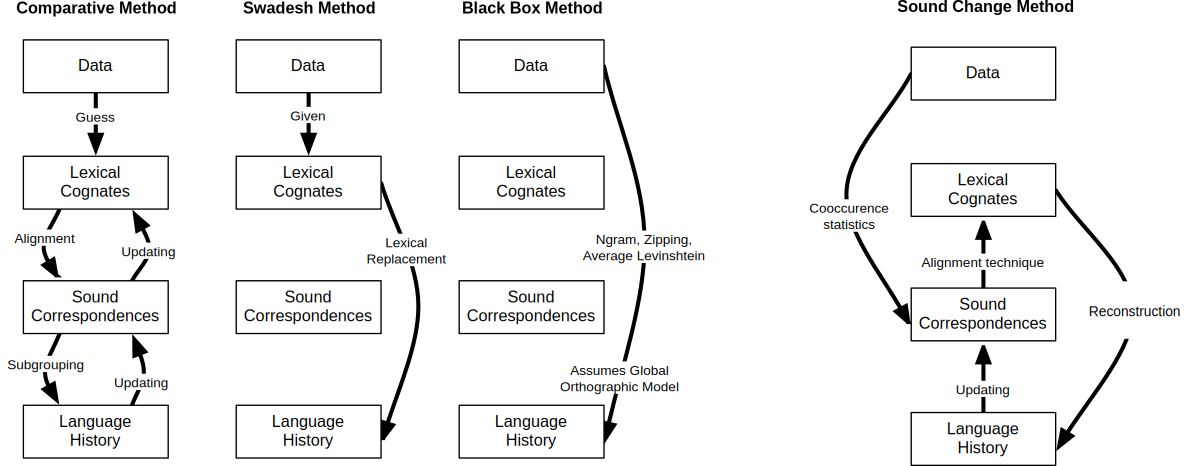
\includegraphics[width=0.9\textwidth]{figures/methods}
\end{center}
\caption{Comparison of workflows to study language evolution. The
  comparative method and the sound change methods are explained in detail
  in the following sections, where we show how those methods produce
  relevant and reliable data. We assume that the traditional Swadesh Method
  is so well known that it does not need to be recapitulated in detail
  \cite{Campbell:1998, Crowley:2010}. Early computational approaches were
  mainly \QUOTE{black box methods}, and merely provided reasonable
  phylogenetic trees without a deeper understanding of the evolutionary
  events and processes explaining the phylogenies they predicted.}
\label{fig:MCyTalk}
\end{figure}

\subsection{IDS as an example of word list data.}

Throughout this manuscript, we will repeatedly make use of word list data
from the \emph{Intercontinental Dictionary Series}~\cite{IDS} to
demonstrate how quantitative method can answer relevant linguistic
questions. Instead of the IDS data, any word list data could in principle
be used.

The IDS word lists are currently available for 241 languages. The set of
languages is regularly extended. For example, Arabic is currently in
progress and has not yet been released at the time of writing. The written
form of the entries varies across the languages. For most languages, a
phonemic-style transcription using IPA, Americanist, or extended Cyrillic
traditions is used. For others an established orthography is used.

All word list are kept in the same format, and the organization is based on
Buck's dictionary~\cite{Buck:49} which was topically subdivided into 23
chapters and had in total about 1200 potential entries for each word
list. The IDS revised the chapter structure such that the IDS word lists
have potentially 22 chapters and in total 1310 potential entries. Entries
for which no word exists in a language are left blank for this
language. Chapters are semantic groups such as \QUOTE{The physical world}
(chapter 1) or \QUOTE{Emotions and values} (chapter 16). Each entry is
assigned to exactly one chapter. Entries within each chapter are roughly
sorted by their semantics, with semantic concepts assigned identifiers of
the form \QUOTE{chapter.meaning}. Both chapter and meaning are numerical
values with the entries within each chapter intuitively sorted by their
meaning.  Furthermore, each entry has translation into English and at least
one additional language, \eg{} Spanish.

In order to bypass manual cognate identification as the initial step one
may start with a much more accessible set of data, namely comparative word
lists not yet subjected to etymological analysis
(Fig.~\ref{fig:MCyTalk}). These compile, for a collection of languages,
words with roughly corresponding meaning, but make no effort to single out
cognates, let alone to distinguish borrowings from vertical inheritance.

The core or basic vocabulary \DB{remove reference to Swadesh list: comprising the Swadesh concepts} when compiled
into such word lists is particularly suited for the phylogenetic enterprise
for two reasons. First, it is composed of many items of proven genealogical
persistence \cite{Calude:2011}, with some of them potentially conserved
beyond the conventionally assumed 10,000 ybp limit of the comparative
method \cite{Pagel:2013}. 
\NEW{Even though Swadesh lists offer an initial starting point, the manner
in which they were created and compiled had its shortcomings \cite{Hoijer:56}}
\TODO{These studies do not "prove genealogical persistence", they are circular in
this respect since they assume families established on the assumption of
genealogical persistence of the very same vocabulary items...} \DB{I agree - however, do we really need this whole section on IDS? I don't think so IMHO}
Lexical replacement rate seems to be linked to
frequency of use, which is fairly comparable, at least across languages
from the largest lingustic families in the world
\cite{Calude:2011,Calude:2014}. Similarly, basic vocabulary is composed of
the lexical elements that are the most resistant to borrowing
\cite{Haspelmath:2009}. For all these reasons, \textit{ceteris paribus},
basic vocabulary items are often considered to provide a more reliable
phylogenetic signal than other non-basic elements. 

As we shall see below, it is possible to extract very good approximations
to cognate sets from such data. Importantly, though cognate judgments made
purely from the phonetic structure captured in these semantically aligned
word lists can be improved with specialized linguistic knowledge, in recent
tests on \QUOTE{simple} language families, the difference was found to have
no systematic structure that could bias the reconstruction of phylogenies
based on this data \cite{Steiner:11a,Hruschka:14}.
\TODO{Rephrase from Importantly on.}
\NEW{For a comparison of different cognate detection algorithms 
see~\citet{List:17}.}

Nevertheless, it is difficult to overemphasize the importance of carefully
curated data sets that are accurate, reliable, uniformly transcribed, and
correctly glossed. Such cleaning of data and making them digitally
accessible needs specialized linguistic knowledge and is time
intensive. One may argue that one can avoid this step because pattern-free
isolated errors in data are unlikely to confound major results. This would,
however, be a mistake when the computation is expected to produce
fine-grained results or is dealing with weak signals. This is the case, for
example, when one is interested in time depths at the limit of resolution
of these methods, or when many threads of intense \TT{areal} contacts need
to be disentangled from each other and from \TT{vertical} transmission. In
what follows, we will always assume that the data has been curated to the
degree appropriate for the resolution required of the results, and
comparable encodings of the wordlists and similar meaning assignments are
used consistently.

\subsection{Identifying  similarities.} 
\label{sec:scoring}

\subsubsection{Word alignments and their scoring.}

The first ingredient in determining historical relatedness of languages is
a means of measuring the similarity of words. Human languages form words by
a combinatorial composition of a basic repertoire of sound-tokens, called
phonemes, that vary between languages. To be useful, computerized word
lists need to encode the phoneme distinctions accurately using distinct
characters; they often also record additional phonetic differences that are
linguistically unimportant in identifying the words or under-represent
crucial distinctions. A related issue is that transcriptions often use
digraphs for single segments, and their usage is sometimes inconsistent
across the orthographies used for the various languages and various sources
of data, even after unicode normalization. Thus, for example, an ejective
may be denoted by superposed apostrophe \NEW{$<$}\'k\NEW{$>$}, postposed
apostrophe \NEW{$<$}k'\NEW{$>$}, postposed palochka \NEW{$<$}k$|\NEW{>}$,
or special letters \NEW{$<$}\cmr\texthtk\NEW{$>$}. Depending on the
encoding, these might be represented either as digraphs or unigraphs. If
the language specific segmentation is available in the data source, these
can all be converted to special characters---\eg{} in the private unicode
space---before analysis. Most often, however, such information is missing
from composite data sources and one chooses a suboptimal solution of
leaving these as a sequence of characters to be handled later. \PFS{An
  example for how to solve this issue will be discussed in section
  \ref{sect:QuRegCh} below.}
 
\par\framebox{\begin{minipage}{0.9\textwidth}\small
\textbf{Discussion of comment: delete when resolved!}

\LM{An example for how to solve this issue will be shown later in this
  section.}  \TODO{Leaving the sequences of characters to be handled later
  leaves the reader wondering, at this point in the paper, how this will be
  resolved. A reference to where it is resolved would be useful.} \DB{I
  would change the last two sentences for a final reference in the previous
  sentence: "before analysis (although chances are such information is
  missing from composite data, which requires different strategies,
  ref. CHAPTER)}
\end{minipage}}  


A very natural starting point, then, is to regard words as sequences of
characters that correspond, at least approximately, to phonemes. The most
direct approach to comparing sequences starts by aligning them. In
bioinformatics, alignments are a nearly ubiquitous first step in
comparative sequence analysis, so that efficient algorithms and ample
experience can be imported from this field. In fact, such techniques for
character-based alignments of words have been used to measure similarity,
\eg{} by \citet{Kondrak:00}, \citet{Cysouw:07}, \citet{Kondrak:09}, and
\citet{Steiner:11a}.

In contrast to the world of biological sequence analysis, where scoring
systems are relatively simple and the algorithmic problems of efficiently
computing alignments of large data sets dominate \cite[see,
e.g.][]{Notredame:07}, it is the construction of good \TT{scoring models}\LM{,\ie{} a function or look up table providing a measurement for the similarity or distance of observed phonemes/characters,} that
is most difficult in language comparisons. 
\TODO{his is the first mention of the term "scoring model" in this section, 
I believe. Because this is a very important concept
for this section I recommend that you introduce it in caps (in keeping 
with other technical terms), and provide a brief definition. Alternatively
the term could be introduced in the first paragraph of the sub-section, 
since it is indeed the focus of this sub-section.}
The fundamental reason for this
is that unlike phonemes, the elementary tokens of biological sequences are
uniquely identifiable across the taxa; for amino acids this is rooted in
their distinct, functionally salient, chemical properties, and for
nucleotides it follows from the extremely slow change of the genetic code
over evolutionary \NEW{time}. In languages, on the other hand, the phonetic
representation of the corresponding phonemes is the fastest process of
change, and needs to be inferred from the data. If alignments of the
cognates were known \textit{a priori}, one could simply use log-odds ratios
of co-occurrence counts as the scoring model.

\begin{figure}
\centering
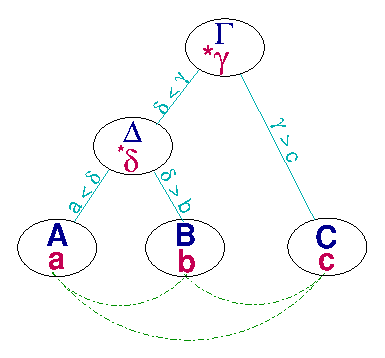
\includegraphics[width=0.5\textwidth]{figures/soundChangeLaws_vs_scoringModels.eps}
\caption{A hypothetical language tree for 5 (proto-)languages (dark blue)
  and one (proto-)sound (pink). Greek letter\NEW{s} correspond to reconstructed
  proto-languages and proto-sounds and Latin letters to the observed sounds
  and languages. Sound change laws (typically used by linguists, turquoise)
  and scoring models (used in quantitative methods, dark green) describe
  both changes between languages in sounds/characters. However, while sound
  change laws describe the changes in the sound system from the ancestral
  language to the descending language, scoring models describe the
  cumulative effect of the sound changes in the languages under
  investigation. For example, the scoring model (dashed-dotted lines) would
  state that $a$ from language $A$ is often found at those positions in the
  words where language $B$ has sound $b$. It thus indirectly \NEW{implies} that $a$
  and $b$ originate from the same proto-sound. The sound change laws
  (straight lines, i.e. branches of the language tree) would state that
  there is a proto-sound ${}^*\delta$ which changed into $a$ in language
  $A$ and $b$ in language $B$.}
\label{fig:ScoringModels}
\end{figure}

It is important at the outset to distinguish the two related concepts of a
scoring model for alignment and the laws of sound change. The score between
character $a$ in language $A$ and character $b$ in language $B$ indicates
$a$ and $b$ form a match in an alignment of two cognate words. Thus it
quantifies the likelihood of obtaining $b$ in $B$ in a place where language
$A$ has $a$ as a consequence of the evolution of both $A$ and $B$ from
their common proto-language. No statement is made about whether this
development was a regular correspondence or, indeed, what the proto-sound
might have been. In contrast, the laws of sound change describe how the
changes along the branches of the language tree happen and, more precisely,
how the proto-sounds of the proto-language changed into the sounds of the
languages $A$ and $B$ under investigation. The scoring model therefore
describes the cumulative effects of the sound changes, including
statistically the effects of apparently irregular developments of
individual words. Furthermore, the scoring model subsumes different sound
changes and proto-sounds as long as their end points are the sounds $a$ in
$A$ or $b$ in $B$.

As an example, let us assume that we have three languages $A$, $B$, and
$C$. The proto-language of $A$ and $B$ is $\Delta$ and the proto-language
of $\Delta$ and $C$ is $\Gamma$ as shown in
Fig.~\ref{fig:ScoringModels}. Furthermore, assume that the proto-language
$\Gamma$ has a proto-sound ${}^*\gamma$. The reconstructed sound laws along
the phylogeny are $\Gamma\ {}^*\gamma > \Delta\ {}^*\delta$, $\Gamma\
{}^*\gamma > C\ c$, $\Delta\ {}^*\delta > A\ a$, and $\Delta\ {}^*\delta >
B\ b$. The corresponding scoring model would not know about the
proto-sounds ${}^*\delta$ and ${}^*\gamma$ but would simply assign high
scores to the cumulative effects. Thus, matching $a$ of language $A$ with
$b$ of language $B$, matching $a$ of language $A$ with $c$ from language
$C$, and matching $b$ form language $B$ with $c$ from language $C$ would
receive high scores.

In a scenario more conducive to the analysis of large-scale data sets
without \textit{a priori} known alignments, two approaches have been
developed. The first of them uses a small amount of linguistic knowledge to
create an initial, crude similarity measure to propose a tentative
alignment. The rule can be very simple. \citet{Steiner:11a}, for example,
only discouraged matches between vowels and consonants, disallowed
transpositions (metathesis), and put more weights on identities of
consonants than vowels. Another example is \NEW{is given by} \citet{Heggarty:00}, who
first used the manually curated proto-forms of the words under study to
infer matches, and then counted the number of phonetic and articulatory
features in which the aligned segments differ. It may come as a surprise
that the model of \citet{Steiner:11a}, which is clearly over-simplified,
nevertheless can identify an initial set of cognates between related
languages. In fact, even these weak assumptions are actually unnecessary:
an alternate approach with even fewer assumption described in
subsection~\ref{sec:tanmethod} can be used to infer the initial
alignment. This works because phoneme evolution proceeds through small
phonetic changes, and cognate pairs having a higher similarity score than
two evolutionary unrelated words is a very low bar.

These methods ultimately utilize the strength of regularities in linguistic
correspondence. Even a very rough and simplistic model for sound changes
suffices to identify at least \NEW{a proportion} of the cognate pairs in the data
set. Given the rarity of metatheses, the pairwise alignments of these
cognates preferentially match corresponding sounds with each other.  The
key observation is that all this needs is an enrichment of cognates in the
initial alignments. Even if a fraction of the candidate cognate pairs are
false positives and some of the alignments of cognate pairs are wrong as a
consequence of the oversimplified scoring model, there is enough signal in
the correct alignments of real cognate pairs for the statistical
machinery to identify the more common sound correspondences.
\TODO{What evidence supports this claim that there is sufficient signal 
in real cognate pair alignments for correct sound
correspondences to be identified in spite of some false positives/wrong alignments?} \DB{I agree on that the claim comes across as a bit vague.}

It is interesting to note that the statistical approach accommodates many
linguistic subtleties without explicitly building them into the
method. Although the mapping of consonants to consonants and vowels to
vowels in the \NEW{\TT{pre-alignments}} is a good working assumption, there is at
least one clear set of frequent exceptions: Vowels often correspond to
consonants belonging to the classes often called glides and liquids, such
as [w, j, l, r]. For example, [l] in the French words \textit{plein,
  plaine, place} corresponds to [i] in Italian \textit{pieno, pianura,
  piazza}. These consonants plus a vowel often also correspond to a single
vowel. For example, /we/ in the Spanish words \textit{bueno, puerto}
corresponds to [\cmr{\textopeno{}}] in Italian \textit{bono, porto}.\footnote{The
  /we/ is orthographically $<$ue$>$ in Spanish.} These kinds of cases can
be taken into account by relaxing the consonant-consonant and vowel-vowel
correspondence constraint. At least some examples of this type appear in
pre-alignments that are classified as candidate cognates \NEW{even though
scores were assigned, not trained in this alignment similar to editing 
operations with similarity scores}. Hence in the
second step they are assigned favorable log-odds scores without the need to
model liquids and glides explicitly from the outside.

A more sophisticated scoring model that takes into account the neighboring
phonetic context can also be estimated from the initial alignments of
cognates. Here, we explore the utility of a bigram-based scoring model and
compare it \NEW{to} a simpler model with unigram scores. The idea behind the
computation of the scoring function is the same for both model\NEW{s}. Likely
correspondences of sounds will appear more often than expected by chance in
an alignment of cognate words. This holds true for both unigrams and
bigrams. In either case we therefore start from the collection of all
alignments of the cognate candidates identified in the pre-alignments of
the word list candidates for a pair of languages $A$ and $B$. For each pair
of sounds $\alpha$ in language $A$ and $\beta$ in language $B$ (where
$\alpha$ and $\beta$ can be unigrams or bigrams as well as gap symbols) we
compute their occurrences $occ_A(\alpha)$, and $occ_B(\beta)$ in the
pairwise alignments. Similarly, we determine the co-occurrence
$occ_{(A,B)}(\alpha,\beta)$, \ie{} we count how often $\alpha$ and $\beta$
appear in the same alignment column of the pre-alignment of the languages
$A$ and $B$. The next step is to convert the occurrence counts into
relative frequencies $p_A(\alpha)$, $p_B(\beta)$ and $p_{(A,B)}(\alpha,
\beta)$. In a random alignment of unrelated words we would expect
$p_{(A,B)}(\alpha, \beta)=p_A(\alpha)p_B(\beta)$. Statistically speaking,
$\alpha\in A$ and $\beta\in B$ are likely to be related if they occur more
often together in an alignment than expected. It is customary, therefore,
to define the score as
\begin{equation}\label{eq:score}
  \sigma_{(A,B)}(\alpha, \beta) = \log\left(\frac{p_{(A,B)}(\alpha,
      \beta)}{p_A(\alpha) p_B(\beta)}\right).
\end{equation}
This so-called log-odds score is theoretically justified by a simple model
of independent evolution \cite{Durbin:98,Altschul:10} \NEW{if there is enough
data for training}.

\begin{figure}
\begin{center}
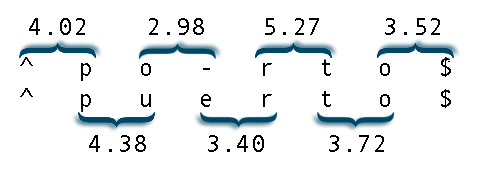
\includegraphics[width=0.35\textwidth]{figures/aln_porto-puerto}
\end{center}
\caption{Example alignment for words from \NEW{Italian and Spanish}
  representing the concept \NEW{\QUOTE{port}}. Each bigram pair in the alignment
  is scored separately, resulting in a total score \NEW{$\sigma=27.29$} in this
  example. Thus the normalized score is
  \NEW{$\textit{nscore}=27.29/(8-2)=4.55$.}}
\label{fig:aln}
\end{figure}

Character-based, \ie{} unigram alignments of words have been described
repeatedly in the literature \cite[see,
e.g.][]{Kondrak:00,Cysouw:07,Kondrak:09,Steiner:11a}. The alignment is
often computed by means of a recursive scheme known as dynamic programming
in computer science. The same idea readily extends to bigrams. Since the
syllable structure is rarely known, it appears prudent to consider
\emph{all} bigrams, and since the beginning and the end of words are often
subject to different sound changes, it is desirable to treat them
separately. The bigram scoring algorithm can be easily extended to handle
this by introducing two additional symbols, \textasciicircum{} and \$,
before the first and after the last character of each word. Thus the word
$w =$ \textasciicircum{} $w_1 w_2 w_3 w_4 \$ $ of length $6$ (four
characters along with the word beginning and end markers) consists of the
$5$ bigrams \textasciicircum{} $w_1, w_1 w_2, w_2 w_3, w_3 w_4, w_4 \$
$. An example of an alignment and its scoring is shown in
Fig.~\ref{fig:aln}. From an algorithmic point of view, bigram alignments are
a fairly straightforward generalization of the well known Needleman-Wunsch
algorithm~\cite{needleman:70} used to solve unigram alignments (see
\hyperref[AppA]{Appendix A}).

\TODO{The text and formulas here are ambiguous as to whether sigma and
  nscore are defined of a pair of languages or a pair of words from
  two lgs.  Presumably the latter but actually the sigma formula as
  written contains free variables that ranged over the full set of
  pairs between two languages on the previous page. Formulas are used
  for clarity so please be explicit as to what is defined over what
  and the domains of free variables.}  Based on this, one can proceed
to define the total score \LM{of two words $u$ from language $A$ and
  $v$ from language $B$ $\sigma(u,v)$} as the sum of all bigram scores
\LM{of all aligned bigrams}
$\sigma(u,v) = \sum_{\alpha \in u, \beta \in v, \alpha\text{ aligned
    to }\beta} \sigma_{AB}(\alpha,\beta)$ together with the
contributions of all gaps\NEW{,\ie{} insertions or deletions of
  characters}, and then a normalized score (\textit{nscore}) obtained
by dividing $\sigma$ by the number of score contributions. \LM{Note
  that the similarity score $\sigma_{AB}(\alpha,\beta)$ for bigram
  $\alpha$ from language $A$ and bigram $\beta$ from language $B$ is
  defined in the scoring model.} In the case of bigram alignments this
amounts $\textit{nscore}=\sigma/\ell$, where $\ell$ is the length of
alignment without \textasciicircum{} and \$. Such a normalization
makes alignments of words with different lengths comparable by
reporting an average score per aligned position.  \TODO{The reader may
  be left wondering about situations where one sound/symbol in
  language A corresponds to two in language B (e.g. Spanish puerta -
  Italian porta, or instances where two symbols correspond to a single
  sound in one language). This is one of the reasons that I recommend
  consolidating the discussion of representational issues and being
  more explicit about what "gaps" are in this method.}  \NR{For this
  todo maybe point to Fig.~\ref{fig:aln}? maybe I can find another
  alignment where there is no deletion score used even though there
  obviously is one.}\LM{Would be cool if we could use the examples
  above, e.g. bueno and bono. Do we have an fitting scoring model for
  this?}

\begin{figure}
 \begin{center}
\begin{tabular}{ccc}
  Indo-European & & Guaycuruan\\ 
   \includegraphics[width=0.48\textwidth,clip=]{figures/nscore_unigram_bigram}
   & & 
   \includegraphics[width=0.44\textwidth,clip=]{figures/bi_uni_scores}
\end{tabular}
 \end{center}
 \caption{Distribution of pairwise alignment score for 11 Indo-European
   (Table~\ref{tab:bigramscores}) (left) and 3 Guaycuruan languages (Toba,
   Pilag{\'a}, Mocov{\'\i}) (right) with a simple unigram scoring model
   (left in each panel) and a bigram scoring model (right in each panel)
   trained on the initial alignments obtained with the simple unigram
   scoring model.}
\label{fig:unibigramdist}
\end{figure}

\subsubsection{From alignment scores to cognates.} 

These normalized alignment scores can be used to distinguish cognates from
non-cognates. In Fig.~\ref{fig:unibigramdist} (left), we show histograms of
both the simple unigram scores and the bigram scores for all pairwise
alignments of words from 11 Indo-European languages \LM{(Table~\ref{tab:bigramscores})}.
\TODO{Which 11 I-E lgs and why those (and, not, say, a single pair). This matters
as the results should look quite different for distantly vs closely
related pairs of languages.}
For both scoring
models we observe two clearly separated peaks. The peak on the left,
centered at negative score values, corresponds to alignments of unrelated
words, \ie{} non-cognates, while the peak centered a positive score values
corresponds to cognates. The right panel shows analogous data for the
Guaycuruan language family. Here the separation between cognates and
non-cognates is much less perfect than in Indo-European, but the two peak
structure is still visible.

Note that the peaks are smoother and more clearly separated from each other
when the bigram score is used. The use of the bigram score thus improves
the capability of the normalized alignment scores to distinguish cognates
from non-cognates. This is not unexpected since regular correspondences are
often sensitive to neighboring phonetic contexts, and a large amount of the
context sensitivity can be partially accounted for by looking at one neighboring
sound along with word boundaries. However, neighboring sounds are an imperfect proxy for only some syllable
boundaries (namely, those recoverable from orthographic representations.) In more difficult cases, such as the Guaycuruan example, the
situation is far from perfect. Here the cognates are not completely
separated from the non-cognates by the \textit{nscore} even for \NEW{the} bigram
scoring model. This leaves us with two possibilities: (1) We can seek to
further improve the scoring model. Below we will briefly discuss a few
ideas in this direction. (2) We can accept that the computational method
does not provide us with a perfect way to identify \emph{all} cognates,
\ie{} we are left with a trade-off between false positives (false
cognates: word pairs that are not truly cognates despite their good score)
and false negatives (unidentified cognates: word pairs that we fail to
recognize as cognates because their score is not large enough). The choice
of the threshold is left to us. Depending on the analysis \NEW{for which} such
cognate identification is needed, we may opt for a conservative strategy
and minimize the false positives at the expense of missing some cognate
pairs, or we may choose to be more inclusive and allow some false positives
to sneak in and contribute to disruption of expected patterns at these
later stages. Importantly, however, the automatic cognate recognition path
provides these later stages of analysis not merely with a binary decision
of whether or not a pair is a cognate, but rather with a score that
represents the weight of phonetic evidence in favor of cognacy. 
\TODO{But cognacy is a yes/no property and modeled as such in the work
the authors cite, so the inability to provide a yes/no answer is
incompleteness rather than a virtue.}\DB{I propose to add at the end of this paragraph - see below.}
Any further
deductions obtained from such putative cognates can weight the evidence by
this score, thereby lowering the deleterious effect \NEW{of} false positives.
Alternatively, of course, the permissive cognate list could be
post-processed to identify and remove false cognates based on expert
knowledge, with manual effort being allocated more to cognate pairs with
low scores. Erroneous cognate detection may also result from erroneous or
inconsistent orthography, manual effort may also therefore be useful in
improving the transcription, so that better cognate recognition will be
achieved by the automatic procedure. It is also important to note that
although the choice of the score cutoff is left to the user, it is not
arbitrary. The shape of the score distribution provides quantitative
information on the expected number of false positives and false negatives
for each choice of the cutoff. \NEW{Finally, these scores can be dichotomized into cognate/non-cognate categories to be used with phylogenetic methods that cannot handle graded evidence for cognacy.}

\DB{I propose to remove this comment, which is verbose and does not add anything relevant: We will return to this point again several
times throughout this contribution.}

We have seen that the improved scoring model leads to refined cognate
identification. In principle we could now iterate this workflow again,
using the alignments of the revised cognate pairs to recompute a refined
scoring model. Somewhat surprisingly, \citet{Steiner:11a} observed that the
method converges already after a couple of iterations and only the first
step from a crude pre-alignment to detailed scoring model yields a
dramatic improvement in the accuracy of alignments and cognate
identification.

Further improvements to the scoring model are possible in principle.  In
order to capture more of the correlations implied by the phonetics of the
languages in question it may be desirable to go beyond bigrams to $k$-grams
for $k\ge3$. Such a model would also take care of local transposition 
\TODO{These were assumed to be so few as to negligible earlier in the paper
so that is not much of an improvement. But if it were important to
capture them, k >= 3 is not necessary as adding transposition operations
to the Needleman\NEW{-}Wunsch algorithm still keeps it polynominal.}
and
regular sound changes dependent on longer contexts, or even word harmony
features. The definition of scores described above generalize in a
straightforward manner since the symbols $\alpha$ and $\beta$ may signify
arbitrary combinations of sounds. In practice, however, the sparsity of the
available data is a limiting factor: not all $3$-grams that are possible in
given language will appear sufficiently often in word list data to get
reliable estimates of their frequencies. A possible remedy is to use
\QUOTE{mixed} scoring models that use $k$-grams with variable length
depending on their frequency in the data. Related techniques have been used
in bioinformatics as means of describing sequence patterns
\cite{Begleiter:04}. The use of such methods, and, in fact, the entire
issue of discovering statistically significant contexts automatically has,
to our knowledge, not been explored so far.

\subsubsection{A probabilistic model of lexical evolution.}
\label{sec:tanmethod}

The approach outlined above is designed to represent the relationships
between the observable data as directly as possibly, without making \emph{a
  priori} assumptions \NEW{about} how exactly languages evolve. An alternative
approach is to start by approximating language evolution as a stochastic
process acting on the phonetic and lexical structure of a language. From
the definition of the stochastic process the conditional probability
$P(D|\mathcal{M})$ of the observed data $D$---in our case word lists of a
set of languages---can be computed as a function of a typically large set
of model parameters $\mathcal{M}$. The idea of the maximum likelihood
approach is to find the set of parameters that maximizes
$P(D|\mathcal{M})$, \ie{} the set $\mathcal{M}$ that makes the observed
data the most likely outcome. With this type of modeling, one makes two
fundamental assumptions: (i) the underlying stochastic processes capture
the dominating processes of language evolution and (ii) the observed data
are typical. In practice, the maximization of $P(D|\mathcal{M})$ is
achieved by iteratively estimating: (1) the probabilities of non-regular
sound changes from ancestor to observed phonemes, (2) a table of regular
correspondences and (3) alignments between words across a set of related
languages.

\textit{A priori} the model allows for an arbitrary amount of phoneme
evolution. Just as described in section~\ref{sec:scoring}, one needs to
start the process with an initial alignment. As an example, one can start
with all words in one language that contain a certain phoneme and
identifies the most over-represented phoneme in the corresponding words in
related languages, compared to expectations based on the overall observed
phoneme frequencies in those related languages. It uses these estimates of
excess representation to initialize sporadic sound change probabilities and
a regular correspondence table, and then uses this information to align the
words in related languages. The non-regular sound change probabilities and
regular correspondence table are then refined by looking at only the
aligned positions and the process is repeated until the iteration
converges. This method of alignment was used to obtain the regular
correspondences in the Turkic language family in \citet{Hruschka:14}
(Table~\ref{tab:turkic}). We use the data set used in that paper to
demonstrate that a high fraction of cognates can be correctly found by
choosing an appropriate cutoff for the best alignment score between
randomly chosen words from different languages. The main advantage of using
the Turkic languages as an example is that relatively comparable phonetic
transcriptions were available, the language family has a relatively shallow
time depth \NEW{(so that cognacy is likely to be reflected in the surface form of words)}, and words had already been categorized into probable
descendants of common ancestors, 
\TODO{It should be mentioned that i) the results do not necessarily generalize
to deeper families/cognacy and ii) that cognates in the Hruschka et al 2015
come in sets whereas the method described in the paper identifies
cognates pairwise and may thus give inconsistent results of the type
A is cognate with B and B is cognate with C but A is not cognate with C.} \DB{The issue of non-transitivity seems to be important but I ignore how it is handled. As for the comment on depth, see my proposed text above.}
so that the results could easily be
compared against expert linguistic judgements.

Since cognates are known for this data set, we can compute the sensitivity
and specificity of the cognate assignment for each choice of the score
cutoff value: sensitivity is the fraction of the true positive cognate
pairs with an alignment score at least as large as the cutoff value;
specificity measures the fraction of non-cognates with an alignment score
smaller than the cutoff. Each cutoff value thus yields a pair of
sensitivity and specificity values that quantify how well the score-based
separation between cognates and non-cognates performs. \LM{One can}
summarize the values in the form of the \textit{Receiver-Operator-Curve}
(ROC) shown in Fig.~\ref{fig:DanROC}. 
\TODO{It's more customary to present the f-score of the precision/recall
corresponding to the different threshold values... \LM{replaced 'It is customary to' with 'One can'}}
Each point on the line corresponds
to a cutoff value and is placed according to the cutoff's sensitivity and
specificity in the plot. The diagonal line indicates equal values for
sensitivity and $1-{}$specificity. This corresponds to a completely random
classification. ROCs below this line are worse than random. The closer the
ROC approaches the upper left corner of the diagram the better the
classification works. As a quantitative measure of goodness, one usually
calculates the area under the curve (AUC), which is $1.0$ for an ideal
test. Mathematically, the AUC represents how often the test assigns a
higher score to a random cognate pair as compared to a random non-cognate
pair, and is, therefore, a threshold independent characterization of the
quality of the scoring system. In Fig.~\ref{fig:DanROC} the AUC is
$0.9$.

\begin{figure}
\begin{center}
\begin{tabular}{rcl}
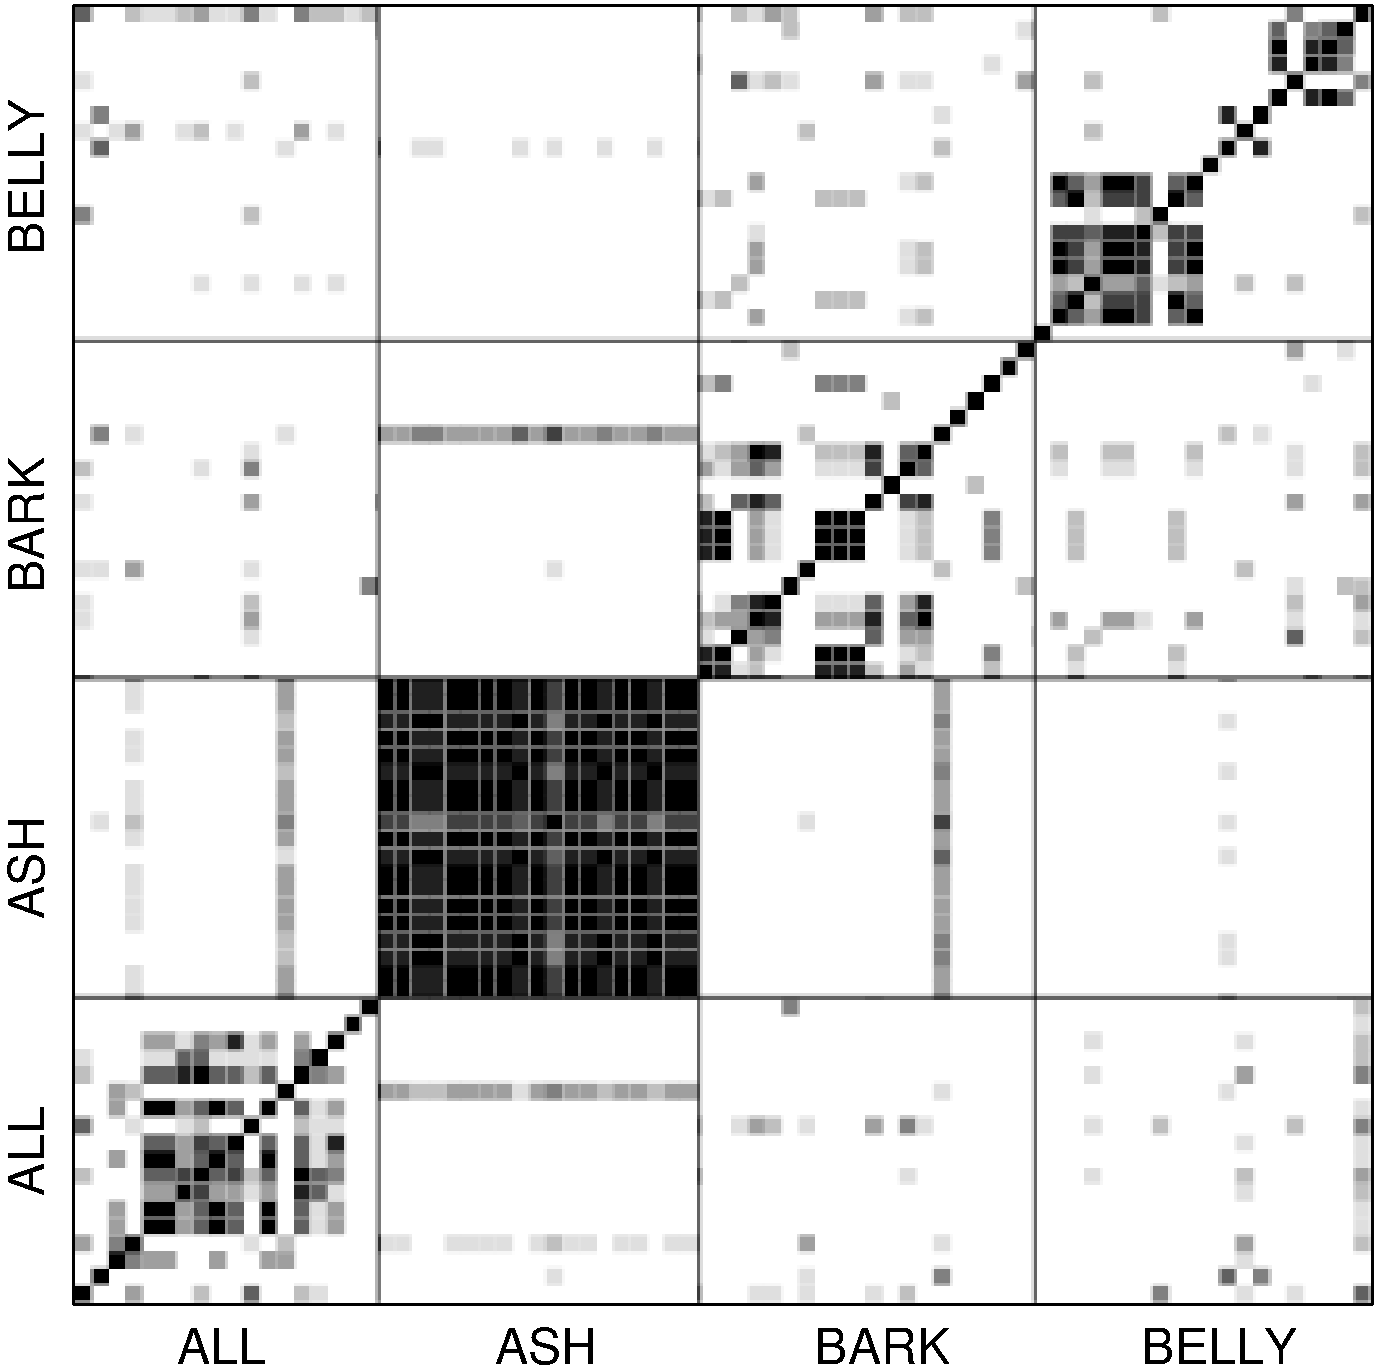
\includegraphics[width=0.45\textwidth]{figures/Hrusch} & & 
\includegraphics[width=0.45\textwidth]{figures/ROCCurve_new}
\end{tabular}
\end{center}
\caption{Aligning words using a likelihood based method can be used to
  detect cognates. Left: Data for 4 Swadesh meanings (all, ash, bark,
  belly) across 20 Turkic languages were aligned and the best alignment
  scores for each pair of words were converted to a distance measure and
  shown as a heatmap: black pixels: small distance between words (between
  $0$ and $2$), white pixels: large distance between words (${}>14$), gray
  pixels: intermediate distances between words (between $2$ and
  $14$). Islands of darker pixels along the diagonal reflect cognate
  classes. Right: An ROC curve for detecting cognates within 50 meaning
  classes in Turkic shows it is possible to find an alignment score cutoff
  with high sensitivity and specificity in separating cognates from
  non-cognates (Area-under-the-curve AUC$=0.90$).}
\label{fig:DanROC}
\end{figure}

The method can, obviously, be refined in ways described in previous
subsections to detect changes conditioned by known phonetic contexts, \eg{}
position within the word, neighboring phonemes or harmony. It is also
possible to weight the commonly used words belonging to the core vocabulary
more than the rare words in deriving the correspondence table, reflecting
the expectation that the \NEW{proportion} of cognates and the regularity of
correspondence is higher in this part of the vocabulary.

\subsubsection{Comparing the two approaches.} 

At face value the two approaches outlined above are quite different. The
focus on alignments and their scores conforms more closely to the paradigm
of sequence comparison in computational biology, while the comparison of
probabilistic models focuses on the evolutionary processes.
Nevertheless, and in spite of these conceptual differences,,
the two methods can answer essentially the same
questions, albeit using different mathematical and computational
techniques and different prior information or expert knowledge.

The likelihood method, for example, does not directly produce a scoring
model. The results are, however, consistent with a scoring model.  First,
it is obviously possible to simply use the alignments to derive a scoring
model as outlined above. Second, one can also use the transition
probabilities between inferred ancestral sounds and their extant
descendants to compute the probabilities of sound correspondences directly
from the underlying stochastic model. Conversely, the scoring system
derived in the first approach does not directly provide reconstructed
proto-sounds. Well understood methods from computational biology are
available, however, to infer ancestral states given observable transition
probabilities \cite{Pennisi:05,Liberles:07}. \NEW{\citet{Brown:13} investigated
the inferrence of sound change rules from a scoring model even though the
direction of the change was not labeled.} Mathematically
this should be possible, however, and we take it on as an interesting open
research question to solve this problem.

In principle, the two approaches can therefore be compared with each other
at all relevant levels: the individual alignments, the inferred scoring
systems, the reconstructed ancestral sounds, and the estimated language
phylogenies. Such detailed comparisons of different computational
techniques are important in their own right since they provide a measure of
sensitivity to the varying assumptions inherent in these methods.

Both methods are alike in that they are almost entirely data driven.  The
alignment scoring, and hence the regular correspondences, are extracted
from the data and represent only information that is contained in the data
set that is actually used in the analysis. As such, one might miss regular
correspondences that are not sufficiently prevalent in the word
lists. Furthermore, the scores are explicitly dependent on the languages
that are compared. Alternative approaches using a scoring system based on
linguistic expertise also exist \cite{Covington:96,Kondrak:03} and such
models could also be designed to be more or less specific for particular
language pairs or language families.
\TODO{Later in the paper sound change processes are argued be universal (a
la Ohala) which means that there is a specific answer to the
incertitude expressed in the above passage.}
\TODO{The "regular correspondences" you refer to here are the same as the 
"table of regular correspondences" you mention on
line 41 of page 12, correct? I suspect that some historical linguists 
will expect that all uses of the term "regular" in relation to sound
changes/correspondences will mean "regular" in the strict Neogrammarian
sense. It would be good to be explicit somewhere in this sub-section
about whether "regular correspondences" does in fact mean "exceptionless" 
as in the Neogrammarian usage.}

\subsection{Phylolinguistics.} 
\label{Sect:SimReg}

\subsubsection{Trees and their reconstruction.}

Decades of practice in bioinformatics, in particular phylogenetics, has
shown that the process of evolution by error-prone propagation of
information very robustly generates tree-like signatures that can be
retrieved from a wide variety of data by means of an equally diverse
collection of methods without the need to have a detailed mechanistic model
of actual processes of evolution~\cite{Waegele:DMP}. Many of these methods
refer to indirect measures such as (dis)similarities, or employ approximate
criteria such as the parsimony principle of cladistics. In fact,
phylogenetics in the pre-molecular era was based entirely on
\QUOTE{characters,} \ie{} descriptions of characteristic features of
organisms. This approach has been tremendously successful without any
recourse at all to an underlying mechanistic theory of character change in
biology. Clearly, it suffices for phylogeny reconstruction that the
underlying evolutionary process causes the divergence of features and that
distinct lineages are affected by changes in an approximately independent
manner. We will return to violations of the assumption of predominantly
vertical inheritance and limitations of phylogenetic reconstruction later
in this section.

%%% 2 

A thorough application of the comparative methods requires the
\emph{simultaneous} estimation of the language history tree, of the
proto-languages corresponding to the interior nodes of the tree, of the
associated regular correspondences, and of the cognates that are invoked in
their support. This amounts to a comprehensive stochastic model of language
evolution. While this approach is certainly the gold standard, it requires
sufficient data to actually parameterize the model with sufficient
accuracy, and sufficient computational capacities.  While this is becoming
feasible at least from a computational point of view, 
\TODO{Reference here is needed to Bouchard-Cote's book but, even more so,
a justification for the totally unspported claim that it is feasible
from a computational point of view is needed...} \NR{no book found}
\PFS{for the ''computationally feasible'' part we can point to the 
  Bayesian phylogeny reconstruction methods and recent methods for 
  reconstruction of ancestral states \cite{BouchardCote:12,Joy:16}
  which solve essentially the same problem in a biological setting.} 

it may not be the
most efficient approach to analyzing the data. In the context of biological
phylogenetics it often pays to subdivide the \TT{gold standard} inference
task into individual components that can be solved independently from one
another.

It is common practice in computational biology to compute sequence
alignments first and to use them as starting point for the reconstruction
of phylogenetic trees. The reconstruction of ancestral
genomes~\cite{Pennisi:05} and ancestral sequences~\cite{Liberles:07} is
then performed on a given tree. Inferred trees may then help to improve
alignments, which in turn yield a better tree in an interative manner.  In
complete analogy, word alignments can be performed independently of cognate
identification and the identification of regular sound changes \NEW{(see 
also~\cite{Kondrak:09})}. One may
meaningfully start by first identifying regular correspondences between
pairs of extant languages and then use the fact that these regular
correspondences are by definition the result of sound changes from the same
proto-language along the two independent lineages to piece this information
together to approximately reconstruct proto-languages and then the
regularities of sound change. 
\TODO{This is an important question, but unfortunately not prudently
discussed in this passage. Since the components depend on each other,
it is not probabilistically correct to do it in the iterative manner,
and, as argued elsewhere in the paper (p 16) it is not a correct
approach from the perspective of propagating uncertainty.}
This separation of tasks is merely a matter
of computational efficiency and expediency. In fact, both maximum
likelihood and maximum parsimony methods necessarily use this kind of
separation internally: likelihoods or parsimony scores are computed for a
given tree, and then used to compare trees. Experience from computational
biology, furthermore, shows that it is often pragmatically favorable to
perform as much of the analysis as possible on directly observable
data. For example, it can be helpful to identify regular correspondences
between extant languages as a first step rather than trying to infer
proto-languages and phylogenetic trees directly.
\TODO{Please explain what experience from computational biology shows how
this is helpful if not for computational efficiency and expediency? As
the text stands this claim is completelty unsupported.} \NR{hab es gedruckt}

Depending on the research question, it is often not even the necessary to
attempt a full reconstruction of language phylogeny. Instead, robust and
reliable statements on language evolution can be derived with much more
modest approaches at both the level of modeling and at the pragmatic level
of computational methodology. For example, hypotheses about the genealogical grouping of languages at different scales
can be proposed on the basis of presence and absence of cognates without
the necessity to model sound changes explicitly
\cite{Bowern:12a,Bowern:12b}.

In the \emph{Classical Comparative Method} carried out manually, a valid
reconstruction is usually interpreted to be a single highly likely
solution. Likelihood based methods, on the other hand, emphasize the
propagation of uncertainties. At its root, a likelihood based method
proposes reconstructions at intermediate nodes and scores the tree based on
the sum of the likelihoods over all possible reconstructions. The
inclusiveness of the likelihood-based approach contrasts with approaches
that have become traditional in manual reconstruction simply through
exigencies of the labor required. To the extent that the data and our prior
knowledge, in a likelihood context, concentrate the support of the
posterior probability on or near a unique reconstruction, likelihood based
methods can be reduced to the traditional interpretation without a
significant loss of their content. On the other hand, when possible
reconstructions are inherently uncertain, likelihood methods propagate the
errors consistently, something that no reconstruction limited to only a
single instance can do. Very similar statements can be made about parsimony
or distance based methods in their domains of validity.

\subsubsection{Beyond computational biology.} 

Despite the conceptual parallels between biological phylogenetics and
phylolinguistics, there are several practical concern that make it
necessary to adapt and modify computational methods from bioinformatics and
computational biology. As a consequence, computational tools from the life
sciences are not readily applicable but need careful modifications and
adaptations. For instance, regular correspondences are inherently
directional and thus non-symmetric, while classical similarity measures are
symmetric by construction. It is easily possible, however, to modify
alignment algorithms so that they can work with asymmetric scoring models,
allowing for the incorporation of directional changes between
languages. Another complication is that while sequence alignments in
bioinformatics can be content with substitutions, insertions, and deletions
as basic operations, additional types of changes appear to occur rather
frequently in language evolution. From an algorithmic point of view the
inclusion of contractions, expansions, and metathesis is
straightforward~\cite{Kondrak:00}; it is a statistical question, however,
when the additional uncertainty arising from the estimation of extra
parameters is justified by the better fit that the model engenders.

Just as in the case of alignment algorithms, there is no reason why the
scoring of trees should rely on symmetric similarity measures. Indeed, a
few recent studies show that regular correspondences can be used just as
well. In~\citet{BouchardCote:13}, for instance, a family of probabilistic
models of sound change is described. These were then applied successfully
to the automatic reconstruction of Proto-Austronesian and its
daughter/descendant Proto-Oceanic. A complete Bayesian approach to tree
reconstruction, incorporating context-independent directional regular
changes, was described by \citet{Hruschka:14}. Similarly, the parsimony
approach used by \citet{Steiner:11a} inherently yields non-symmetric models
of regular sound changes.

Another difference between the phylogenetic problem in computational
  biology and linguistics arises from the nature of the evidence.  Genetic
  material being analyzed comes from individuals in a population, and the
  computed phylogenetic tree is an approximation to the genealogical
  relations between these individuals.  As such, the splits in the tree
  represent survival of sibling lineages in the data set, and do not
  represent moments of special change. In contrast, linguistic material is
  usually a record of a conversational norm in a society. Splits in a
  linguistic genealogy thus approximate to splits in linguistic
  communities.  In this respect, linguistic analysis is more like analyzing
  morphological traits in the biological literature, and language evolution
  parallels evolution of morphological traits in biology. In both systems
  one finds evidence of punctuated evolution \cite{Pagel_rates} as well as
  population size effects on rates of evolution \cite{Bromham:15}.  Similar
  remarks apply to uncritical assumptions about uncorrelated Poisson nature
  of changes in various linguistic features.

  There are additional problems for some Bayesian analyses that try to use
  information about the expected shapes of phylogenetic trees
  \cite{Kingman:82}.  These expectations are based on finite variance
  birth-death models maintaining large populations.  There is no \textit{a
    priori} reason to believe that linguistic community splits will lead to
  similar trees. Nevertheless, Bayesian methods are useful in propagating
  uncertainties and can properly incoporating non-linguistic constraints
  such as arising from known histories of population movements and lack of
  contact over certain time ranges.

  These cautionary remarks apply only to a blind application of
  programs developed for the biological domain to linguistic data.
  What is needed, instead, is a reformulation of the problem for the
  linguistic domain taking into account its particularities. Such an
  approach carries over the mathematics already developed to deal with
  historical processes in biology to this domain without a false
  reduction of linguistic or cultural traits to genetic sequences or
  genes.

\subsubsection{Deep phylogeny and its limitations.} 

Similarity serves only \NEW{as} a first filter for relatedness. In fact, \DB{I propose remove: the rate of
\QUOTE{random} mutations variously} \NEW{the rate of sound change} affecting \DB{I propose remove: the sounds} in individual words
is so low that the method of comparative historical linguistics stipulates
that only regular correspondences can be invoked to support the recent
relatedness of languages. 
\TODO{It is not entirely clear what this sentence means, or how to evaluate 
the claim here without knowing exactly what you
mean by 'random' mutations in this linguistic context. Do you mean 
sporadic changes? Either some clarification or a reference to some supporting
discussion would be very helpful.}\DB{See my proposal.}
But at deeper time scales, not only these
\QUOTE{sporadic} sound changes, but also fusion of morphemes, morphological
analogy, lexical diffusion, frequency effects, dialect mixture, inherent
variations, borrowing from other registers, etc., build up and reduce the
observed regularity. The view of many linguists is that when the cumulative
effect of these intrusive events obscures the regular correspondences,
reconstruction of chronologically deeper families is futile. This is
especially problematic since a desirable, though not strictly necessary,
result of the application of the comparative method is the reconstruction
of a proto-language invariant from which the descendant languages can be
deduced via a set of regular phonetic laws.

A variation has been advocated that reconstructs proto-languages using a
step-by-step reconstruction sequence, where intermediate reconstructions on
a smaller time scale are then compared with each
other~\cite{WhorfTrager:37,Haas:69}. This is useful when due to layers of
accumulated phonetic change, ancestral states of great time depth are not
easily deduced from modern languages, but it throws away possibly
informative information carried in the \emph{variation} of forms within
clades of shallow time depth, not allowing information from sister
subgroups to inform the
reconstruction~\cite{Hockett:58,Greenberg:87,Fox:95}. Instead of choosing
one extreme over another, a probabilistic framework can be designed to
admit effectively irregular changes at a low rate, but favor a regular
explanation when the data demands it.

There are, of course, inherent limits to the resolution of chronologically
deeper branches in phylogeny. All signals that can be used to infer trees
from extant data (e.g. sound changes, lexical replacement, and turnover of
typological features) are necessarily cumulative and therefore will
eventually saturate. Deep phylogeny applications in biology, therefore,
focus on slow-evolving characters and disregard features that evolve at
faster time scales. It is at present not completely clear whether
sufficient phylogenetic signal has been retained by languages in the
different well-established families to disentangle their deep phylogenetic
relationships. This is, however, a question that can be addressed and
answered by quantitative statistical methods in a systematic manner using
the available data sources.

Many key questions of deep phylogeny in biology have recently been
addressed very successfully not only because genome projects have provided
access to much larger data sets for individual taxa but also because
methods have become available to combine different data types from
molecular sequences to detailed morphology character tables
\cite{Waegele:DMP}. Maybe even more importantly, denser taxon sampling
leads to considerable improvements in the quality of phylogenies due to
noise reduction \cite{Zwickl:02}, helping in particular with the resolution
of early branches. Analogous approaches can be envisioned for language
comparisons. The expansion of word list well beyond Swadesh sets, the
integration of slow-evolving language features, and the addition of more
languages together are likely to lead to major progress in deep
phylogenetics of languages. The need for a drastic expansion of the data
sets in phylolinguistics implies that efficient computational methods are
needed to help with preparation and quality control of the input data sets
at an early stage. Thus, for example,  errors in the coding of linguistic data often introduce
rare characters or unusual sequence of characters into the data; a hidden
Markov model could be trained to learn the probabilistic patterns in the
sequence of characters composing the words of a particular language and
extremely rare occurrences of characters or sequence of characters can then
be flagged for manual verification.

\subsubsection{The effects of borrowing.} 

Not all language change can be attributed to vertical inheritance. It is an
important function of a good alignment method to seed language comparisons
with the correct regular sound correspondence, rather than a false
correspondence suggested by borrowed forms. Whether this is achievable, and
how much linguistic knowledge may be required to supplement the data for a
particular comparison, depends on the structure and coverage of available
data from the languages being compared. In particular, extensive contact
and borrowing might make it impossible for purely computational methods to
disentangle vertically and horizontally inherited words. This is also an
issue in bioinformatics, where Hidden Markov Models have been quite
successful in recognizing sequences that have been acquired by horizontal
transfer \cite{Dufraigne:05}. It will remain to be seen whether a similar
approach can also be successful in cases of large scale borrowing.
\TODO{Please explain what this HMM does? (HMM is an extremely general technique
for sequences and it is not obvious how they can be used in the manner
mentioned).}

It is generally believed that the vertically transmitted patterns of sound
\NEW{change} between two language lineages form consistent systems applying
to all or nearly-all words they affect, even if the sounds themselves have
diverged widely. Isolated loan words may show similarities of sound
patterning with other languages, but they should not in general assemble
into a system with the same degree of internal consistency as the system
produced by vertical descent. For example, Russian \LING{molozivo}
\QUOTE{colostrum} is cognate to German \LING{milch} \QUOTE{milk} and shows
more consistency with the regular correspondences, rather than the borrowed
form \LING{moloko} \QUOTE{milk} which is semantically more similar to
\LING{milch}.\footnote{Even in word lists derived from standard orthography
  several automatic regularizations are performed that do not affect the
  detection of sound changes. Among them is the removal of
  capitalization. We report words here as given by the word lists, hence we
  write \LING{milch} \QUOTE{milk} instead of the orthographically correct
  \LING{Milch}.}  In this sense the emphasis on regularity is believed to
reflect more fundamentally the way language structure causes relatedness
due to common descent to be expressed in lexical comparisons. Note that we
use the term lexical comparison to explicitly include the comparison of
phonemes/characters comprising the cognates in addition to the more
traditional analysis of the presence or absence of cognates with a given
meaning. Similarity of non-loanwords can carry information about timescales
in a context defined by the system of regular correspondences. In practice,
however, whether the internal system coherence produced under vertical
descent can be distinguished from \TT{borrowed coherent correspondences}
will depend on the number of words that have been borrowed from individual
sources, the way these are distributed among core and peripheral vocabulary
items, and whether influences on other language features such as morphology
have influenced the use of either vertically transmitted or loaned words.

\begin{figure}
  \begin{center}
    \begin{tabular}{cccc}
      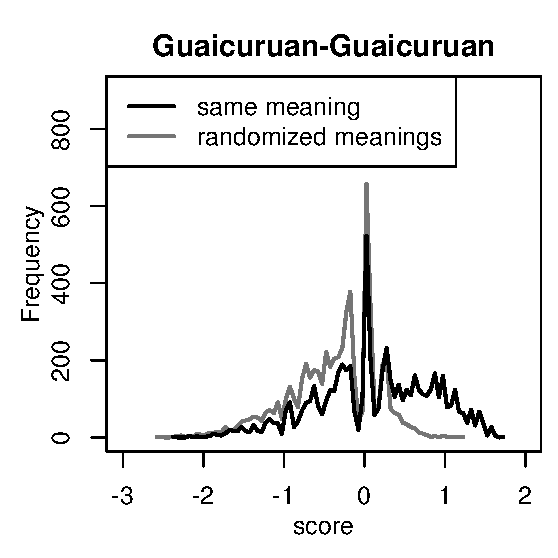
\includegraphics[width=0.21\textwidth,clip=]{figures/G_G}
      &
      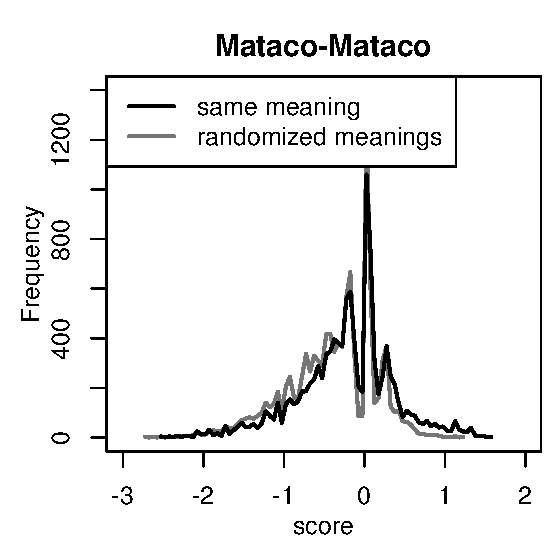
\includegraphics[width=0.21\textwidth,clip=]{figures/M_M}
      & 
      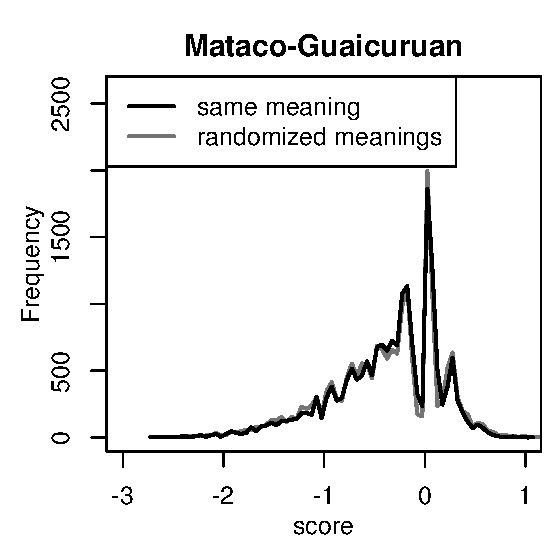
\includegraphics[width=0.21\textwidth,clip=]{figures/M_G} 
      &
      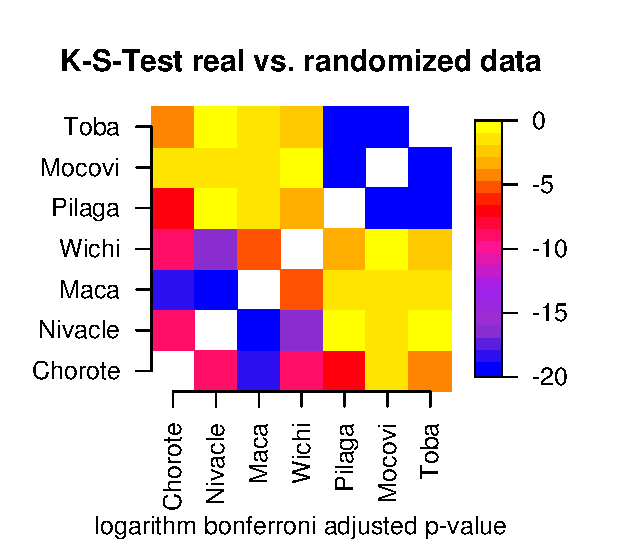
\includegraphics[height=0.21\textwidth,clip=]{figures/bonficols}\\
      (a) & (b) & (c) & (d)\\
    \end{tabular}
\end{center}
\caption{Distribution of pairwise alignment scores for languages from the
  Mataco (Nivacl{\'e}, Maca, Wich{\'\i}, Chorote) and Guaycuruan (Toba,
  Pilag{\'a}, Mocov{\'\i}) languages. In panels (a-c), pairs of words with
  the same meaning according to the input word lists are compared with
  scores for pairs of words with independently randomized assignments to
  meanings. For comparisons within each language family (panels a and b) a
  clear shift to the right is observed for meaning-matched word pairs:
  \ie{} more meaning-matched pairs with large scores are observed compared
  to pairs with randomized meanings. In contrast, the two distributions are
  nearly identical for comparisons of one Mataco with one Guaycuruan
  language. Thus, there is a clear statistical signal for relatedness
  within Mataco and within Guaycuruan, but not between the Mataco and
  Guaycuruan families. (d) In a more detailed analysis, each pair of
  languages is compared separately and the statistical support for the
  difference of distribution is measured by the Kolmogorov-Smirnov test. We
  find strongly supported blocks (cooler colours) within the Mataco and
  Guaycuruan language families, but little signal across the family
  division. Data were recomputed from~\citet{Steiner:11a}. }
\label{fig:permut}  
\end{figure}

\subsection{The virtue of statistical tests.} 

In the last section we sketched the basic tools and procedures that take us
from raw data to the estimate of trees, regular sound changes or
alignments. However, the whole enterprise relies on the assumption that
there is a bona fide phylogenetic signal in the data. Furthermore, we have
listed a few factors that might account for the absence of a such a
signal. It should be \NEW{noted} that the methods discussed before will yield
an answer even if the data at hand is essentially structureless noise---in
other words, the fact that a tree can be produced is not a guarantee that
it bears any meaningful information with respect to genealogy.

For the purpose of distinguishing structureless from potentially
informative data, statistical thinking plays a central role. The key notion
is the \TT{null hypothesis}. Roughly speaking, a null hypothesis is a
scenario or a collection of scenarios where there is no signal in the
data. This would answer the question of \QUOTE{how would a tree, regular
  sound change, or an alignment look like when there is no phylogenetic
  information at all?} The goal is to have a concrete baseline against
which one compares the empirical results: if the results found in the
analysis of data do not differ in any meaningful way from the uninteresting
case of the null hypothesis, then we have no case for our analysis, unless
strong external evidence could be invoked. To give an extreme example, if
we align two series of words from a pair of languages that are believed to
be related and find that their similarities are not so different from what
would be found in a random collection of strings, one has to either drop
the idea of genealogical relatedness, or there must be good arguments
(\eg{} genetic or anthropological data suggesting that the populations were
related) to persist in the quest for genealogical relatedness. Even then,
for such a postulate of relatedness to be entertained, an explanation, such
as a large time depth, for the absence of a signal has to be given.

Let us flesh out \NEW{a concrete example in more detail}. In the case of
cognate judgments based on similarity scores, for example, one could
construct a null model to test that pairs of cognates are more similar than
pairs of non-cognates. Let us assume that we know, for a particular scoring
model that we want to use, the probability $P(s)$ that the score $s$ is the
similarity score of a pair of non-cognates. This distribution, then, can
serve as the null model: if the results we find are comparable to what one
would get with non-cognates, there is little motivation for pursuing the
matter any further. We can then calculate the similarity score $\bar{s}$
for a word pair $\omega$ and ask how likely it is to find such a score or a
more extreme score under the null model, \ie{} under the score distribution
of the non-cognate word pairs. In the case of the similarity scores,
\TT{more extreme} means scores that are even larger than the observed score
$\bar{s}$. Thus, the probability that our word pair $\omega$ has a score of
at least $\bar{s}$ when the words are not cognates is $P(score(\omega) \ge
\bar{s})=\sum_{s\ge\bar{s}}P(s)$. This probability is called the
\TT{$p$-value} and quantifies how likely it is to obtain the observed
similarity score if the null model was true. The smaller the $p$-value, the
more confidence we have that the observed score does not come from the null
model.

A null model can be particularly detailed if we know precisely what the
no-signal case is. In this respect, it can be as complex as the alternative
hypothesis we entertain. However, there are shortcuts to null hypothesis
construction based on the empirical data itself, a prominent example being
\textsc{permutation tests}. The general idea behind a permutation test is
to construct the null model by randomly rearranging the observed data in an
attempt to destroy all the regularities that can be suspected to be related
to the effect under consideration \NEW{(see~\citet{Oswalt:70} for an example
on permutation tests in linguistics)}.

Let us consider again cognacy as an example. Given word lists of two
languages, we expect cognates to be much more frequent among words that
share similar or identical meanings. The corresponding null-model thus
consists of randomized word lists, where words with different meanings are
matched across languages \cite{Baxter:00}. If meaning-matched words are
more similar to each other than words from unrelated meanings---ignoring
horizontal transfer and sound symbolic shared patterns
~\cite{dingemanse2015}---a statistically significant difference between
real and permuted similarity distributions supports a non-trivial
genealogical relationship between the languages.
\TODO{This idea is limited by regularities in the meaning space of the kind
discussed in 4.1-4.2 (as well as synonyms). The paper would make an
actual contribution if this was taken seriously for a correct
assessment of number emanating from a permutation test.} \DB{This is more work...}


The data
is again taken from the IDS. For each language, we have about 1000 words in
the word list and unique identifiers for the meanings across all word
lists. We took the similarity scores from~\cite{Steiner:11a} and calculated
the similarity of a word pair as the alignment score of the best alignment
between the two words with respect to the scoring model. While this can be
done in theory for all word pairs, we only chose word pairs with identical
meanings originating from different languages. Furthermore, we split up the
data into alignments within Mataco, within Guaycuruan, and between Mataco
and Guaycuruan. The distributions of the scores, \ie{} the frequency of
each score, is then shown as black lines in Fig.~\ref{fig:permut}
(a)--(c). The entire procedure was then repeated with the permuted word
lists. As explained above, the permutation is performed by re-assigning
each word of the language to a meaning randomly and independently for each
language. In this way, we measure how much similarity we would expect
between words that typically do not have the same origin, \ie{}
non-cognates. In other words, we estimate the \TT{null model} for the score
distribution and show them as superimposed gray lines.

If we now want to answer the question of whether there is a non-trivial
relationship between two languages, we need to test whether the score
distribution of the real data is different from the score distribution of
the permuted data. For this purpose we performed a Kolmogorov-Smirnov test
\cite{Smirnov:1948}, which basically tests the null hypothesis that the
difference in distributions is only due to sample-to-sample fluctuations
expected of finite samples. Once more, a small $p$-value hints to the fact
that the null hypothesis is a bad assumption for the data at
hand. Therefore, we performed the test for each pair of languages in the
data from the Mataco-Guaycuruan group of languages and obtained a $p$-value
for each language pair. Recall that the $p$-value measures how likely it is
that we obtain a value at least as extreme as the observed. As we discussed
before, if a single test is performed, small $p$-values suggest that the
null hypothesis might not fit the observed data well. If several
statistical tests that produce $p$-values are performed instead, then
naturally from time to time a system that complies perfectly to the null
hypothesis will yield a small $p$-value.

Therefore, one has to correct the $p$-values of the $m$ independent
tests. In our example, we have $7$ languages and thus $30$ different
language pairs. 
\TODO{Is the math correct here? 7 x 6 / 2 = 21 according to me.}
To illustrate the problem, let is consider $0.1$ as our
significance cutoff for the $p$-value. Then the probability that we call a
result significant even though it is not, is exactly the $p$-value and thus
at most $0.1$. Now if we observe all $30$ $p$-values from the 30 tests are
$0.1$, we can still correctly conclude that for each test the chance to
call the result significant, if it is not, is $0.1$. Vice versa, the
probability that a test classifies the result correctly as significant is
$0.9$. Consequently, the probability that all $30$ test classify the
results correctly as significant is $0.9^{30} = 0.04$, which leads to the
conclusion that the probability that we call at least one insignificant
result as significant is $1-0.04=0.96$. In other words, even though we find
30 significant $p$-values, it is very likely that at least one out of 30
test is incorrectly identified as being significant. A traditional way to
correct for this effect, known as multiple testing problem, is the
Bonferroni family-wise correction~\cite{Bonferroni:1936} which simply
multiplies the $p$-values with the number of independent tests $m$ or,
equivalently, divides the cutoff by $m$. The Bonferroni correction is
extremely conservative and other methods of correcting for multiple testing
also exist in the literature, and may be used in cases where we have more
tolerance for false positives~\cite{Holm:1979, Hochberg:1988, Hommel:1988,
  Benjamini:1995, Storey:2002}.
  
We depict the corrected $p$-values in Fig.~\ref{fig:permut}(d) as heatmap
where yellow corresponds to the highest possible $p$-value of $1$ and blue
corresponds to the lowest observed $p$-value of $10^{-20}$. We can see that
there is a very strong signal of relationship within the group of
Guaycuruan languages. Also within the Mataco languages, we observed a
significantly strong signal. Thus, for both groups we obtained the signal
and can conclude that the languages have a relationship stronger than
expected. Between Mataco and Guaycuruan there is, if at all, only a weak
signal between Chorote and Pilag{\'a}. Thus, a non-trivial relationship
between Mataco and Guaycuruan is not supported.  While the results in this
case are not surprising, they nevertheless demonstrate the power of
permutation tests and statistical testing.

Of course, the usefulness of permutation tests depends on the quality of
the test statistic. In our example, how well does the measure of word
similarity represent the true relationship? The better the numerical value
of similarity correlates with evolutionary distance, the more sensitive
will the results of our test be. Thus, a similarity measure that depends on
inferred patterns of regular correspondences is likely to provide a better
inference of genetic relationships than a similarity measure that depends
only on shared sound features in individual words. Nevertheless,
statistically, any permutation test that gives a statistically significant
result, after correcting for the number of independent tests performed,
points to a non-random underlying process.

Both, the permutation test and the test of significant difference in the
distributions, are model independent. In the case of the test for
difference in the distribution just the empirical data is used without
making any assumption on the underlying theoretical distribution of the
data. Consequently, the Kolmogorov-Smirnov test can be used even if the
theoretical distribution is unknown.

\begin{figure}
\begin{center}
  \includegraphics[width=0.5\textwidth,clip=]{figures/fdrcurves}
\end{center}
\caption{Estimates of the false discovery rate as a function of the
  predicted cognates for three pairs of languages. As the score cutoff
  $\theta$ decreases with the number of predictions, the FDR increases
  approximately monotonically. For the closely related Pilag{\'a} and Toba
  hundreds of cognates can be identified without much danger to make
  mistakes. Larger cognate sets for the related, but much more diverged
  languages Chorote and Nivacl{\'e} cannot be extracted without
  contamination by false positives, roughly 20\% within the top 100
  predictions. For the presumably unrelated languages Chorote and Pilag{\'a},
  the FDR increases even more rapidly.}
\label{fig:FDR}
\end{figure}
%
The results of permutation tests in our example have another immediate use,
namely the identification of likely cognates. Retaining only those word
pairs with a similarity score larger than some cutoff $\theta$ provides a
set of candidate cognates. The randomized distribution tells us how many
false positives (namely how many unrelated pairs of words are incorrectly
classified as cognates) we have to expect at this level of similarity,
namely as many as the number of pairs with a score larger than $\theta$ in
the randomized distribution. In the examples in Fig.~\ref{fig:permut}, we
find virtually no expected false positives for scores above $\theta=1$. As
the cutoff is lowered, we expect to find more true positives, but only at
the expense of a contamination of the candidate set by false positives. A
common way to control this trade-off is to determine the false discovery
rate (FDR), that is, the fraction of positive test results that are
incorrect. The set of word pairs with a similarity ${}>\theta$ will contain
both correct cognate pairs and incorrect ones. Since it is plausible to
assume that word pairs from two different meaning categories will rarely be
cognates, we can estimate the number of false positives as the number of
word pairs with a similarity ${}>\theta$ after randomizing the assignment
of words to meanings. Fig.~\ref{fig:FDR} shows how the FDR increases with
number of predictions. The acceptable level of the FDR depends of course on
the purpose of the study. In many cases an FDR of $0.1$ is often deemed
acceptable but a more stringent value may be desirable, for instance, to
limit the predicted cognate pairs to a number that is managable for an
expert linguist to carry out an in depth analysis on.
 
\begin{figure}
\begin{center}
  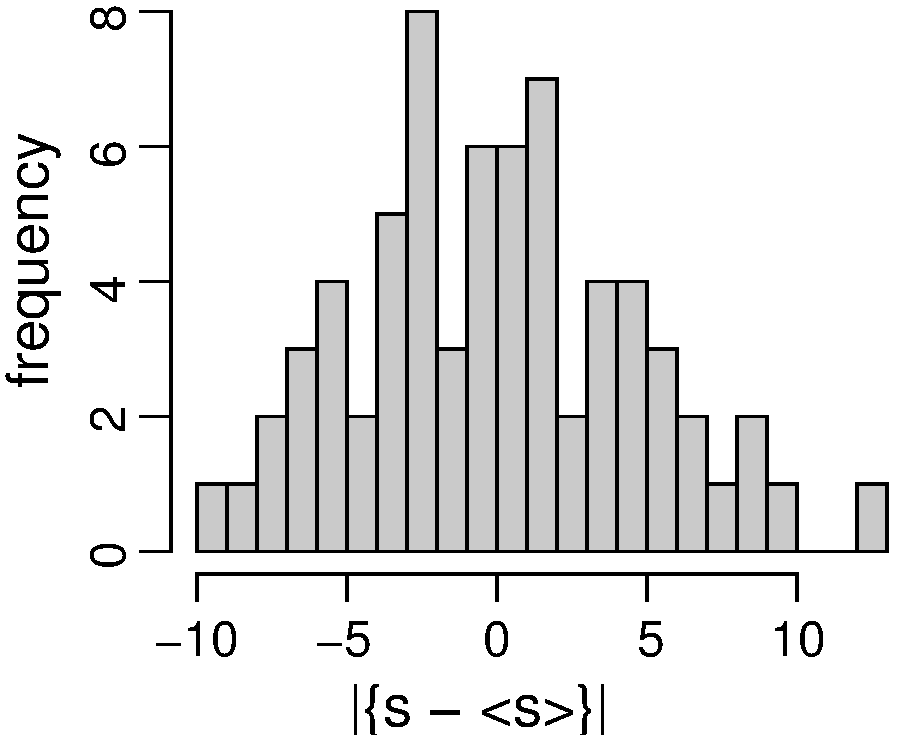
\includegraphics[width=0.5\textwidth,clip=]{figures/CH_new}
\end{center}
\caption{Comparison of 70 South American languages with English. The
  histogram shows the number $s-\langle s\rangle$ of words that are more
  similar than the randomized baseline.}
\label{fig:Chist}
\end{figure}

Fig.~\ref{fig:Chist} shows an example of an expected negative result. To
check if there is signal of similarity between English and South American
languages, we compute for each language the number of words of the same
meaning that are more similar to English than the background similarity
estimated by randomizing the assignment of meanings. The symmetric
distribution around $0$ shows that there is, as expected, no signal. The
power of statistical testing, however, lies in the fact that a
Kolmogorov-Smirnov test as described above can be used to assign this
conclusion a precise evidentiary value characterized by the $p$-value of
the test.

\subsection{Quantifying regular change: the importance of representation.} 
\label{sect:QuRegCh}

The ease with which sound similarities or regular correspondences can be
discovered depends on the encoding used to represent the sounds of the
language. For languages with a single dominant script, one can choose to
use the established orthographies; but this is often not an ideal
representation. Scripts and languages are often inherited from different
sources, and orthography often encodes orthographic history, in addition to
current distinctions. It also frequently fails to indicate important
distinctions, or represents distinct sounds in ambiguous ways.  Finally,
many writing systems do not directly encode the phonetics at
all.

Using a fine-grained, subphonemic, transcription to represent the
pronunciation accurately brings its own set of problems. Phonetic detail
plays a role not only in distinguishing different words, but also to signal
emotions, status and ethnicity. These differences lead to individual speech
variations much of which can be represented in a sufficiently fine grained
phonetic markup.  Linguistically, however, the sounds that we are often
interested in analyzing are the ones that contrast different lexical
items. The overloading of the phonetic medium for carrying both linguistic
meaning and extra-linguistic signals, and lack of strong constraints from
an underlying physical substrate, naturally leads to a
\TT{virtualization}~\cite{Doyle:11}, where the perceptual tokens map onto
speech sounds in a labile but rule-directed fashion. Since these tokens, or
phonemes, are the linguistic building blocks for lexical items, a word list
encoding only the phonemic structure can retain the linguistically salient
sound differences removing the less useful variation. A phonemic
transciption is also useful in erasing \TT{allophonic} phonetic differences
that are completely predictable from neighboring phonetic structure. Such a
structure also has the advantage of making similarities and regularities
across languages easier to detect.

Of course, it can be argued that the different sound values carried by each
phoneme in closely related languages also provides information that can be
used to measure the amount of divergence between the languages.  Analysis
of such data sets based on similarity alone is often difficult, without
projecting to a representation that erases small but frequent phonetic
shifts. On the other hand, if the data set is large enough to parameterize
a sound change model and evaluate its goodness of fit, the information in
such fine grained data can be properly used.

In summary, to find the relations at a certain depth, it is useful to
encode the sounds in a system that erases distributional distinctions that
are important at a shorter time scale but preserve slowly varying features
that are useful for the classification.

To demonstrate that effects of different encodings is small we consider two
examples. First we test the effect of minor inconsistencies between
transcription systems. To this end we selected Mocov{\'\i} and Pilag{\'a},
two of the three Guaycuruan languages also used for the analysis shown in
Fig.~\ref{fig:permut} and artificially introduced some changes that mimic
different interpretations of phonemes. We used the original data of
Mocov{\'\i} from the IDS database and replaced [i] by [e], [k] by [c], and
exchanged [a] and [o]. Thus, while in the initial encoding [a] of
Mocov{\'\i} and [a] of Pilag{\'a} were likely the same sound, in the
artificially recoded data this is not longer the case. In addition we have
erased the difference between [k] and [c], and [i] and [e],
respectively. We prepared two data sets. One data set contains Pilag{\'a}
and the Mocov{\'\i} in the encoding provided by the IDS. The other data set
contains Pilag{\'a} and the artificially recoded wordlist of
Mocov{\'\i}. For both data sets, we trained a bigram-model as described
above and obtained pairwise alignments with the trained bigram-model. It is
important to note that the score values are not directly comparable between
different data sets. We therefore used permutation tests on each data set
to obtain the score-cutoff that corresponds to an FDR of 10\% and used
these score cutoff values to make the cognates assignments for each
dataset. Then we compared the results between the native and the
artificially recoded set. We found that 97\% of the cognates pair called in
at least one data set, are also called in both cognate sets (see
Fig.~\ref{fig:encoding}a).
\TODO{The final sentence of this paragraph needs to be reworded for clarity.}

\begin{figure}
  \begin{center}
    \begin{tabular}{cc}
      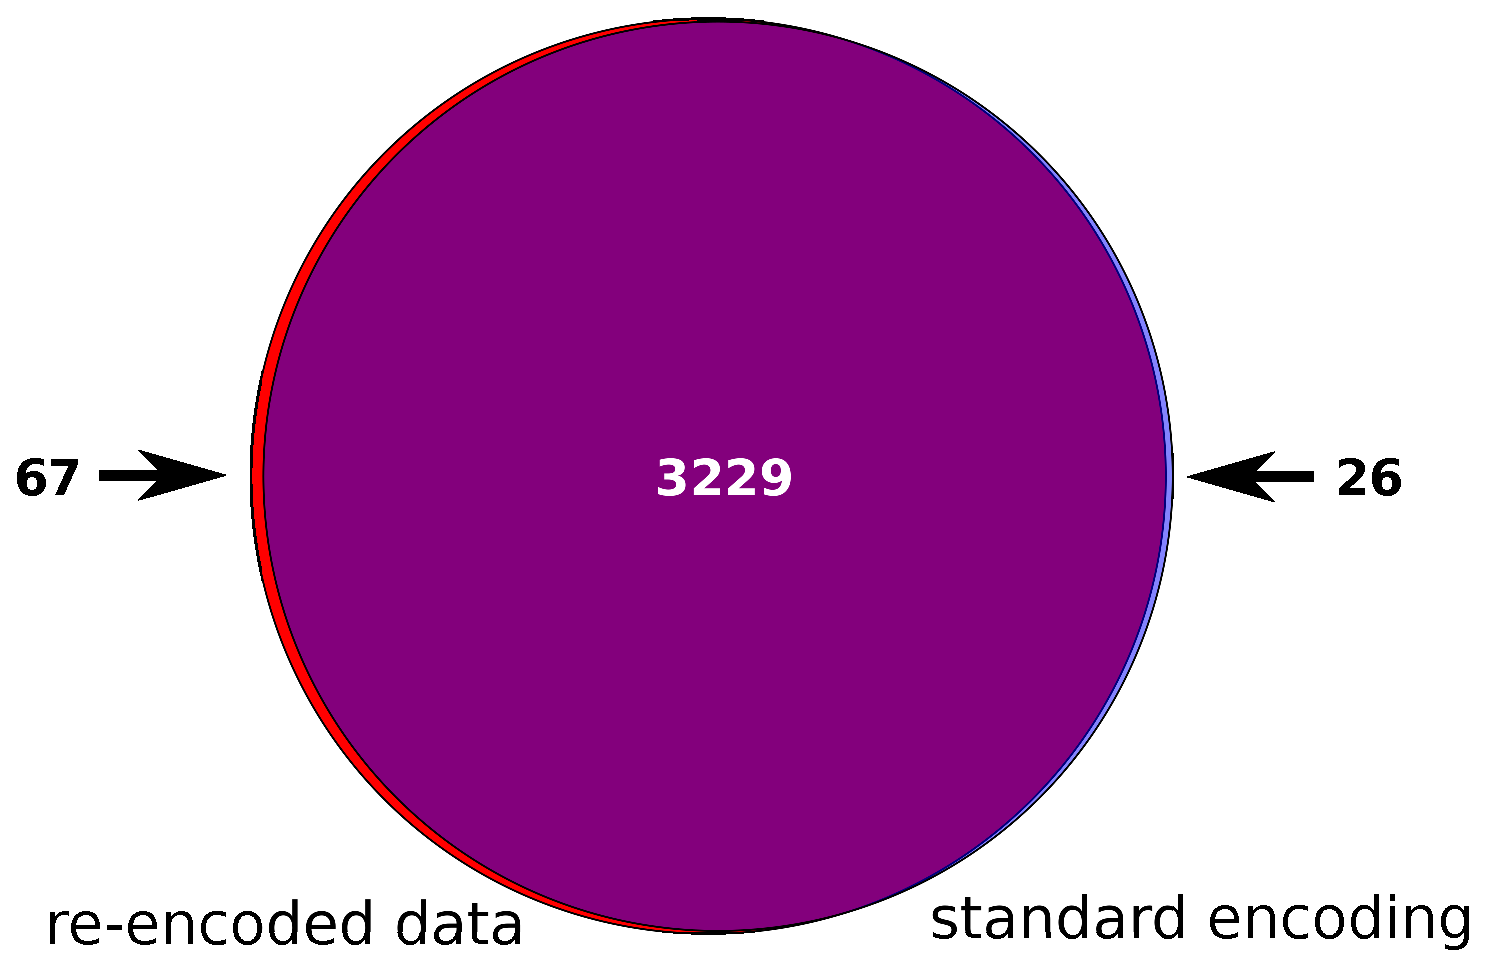
\includegraphics[width=0.45\textwidth,clip=]{figures/pairwiseVenn_sameMeaning_0_1}&
      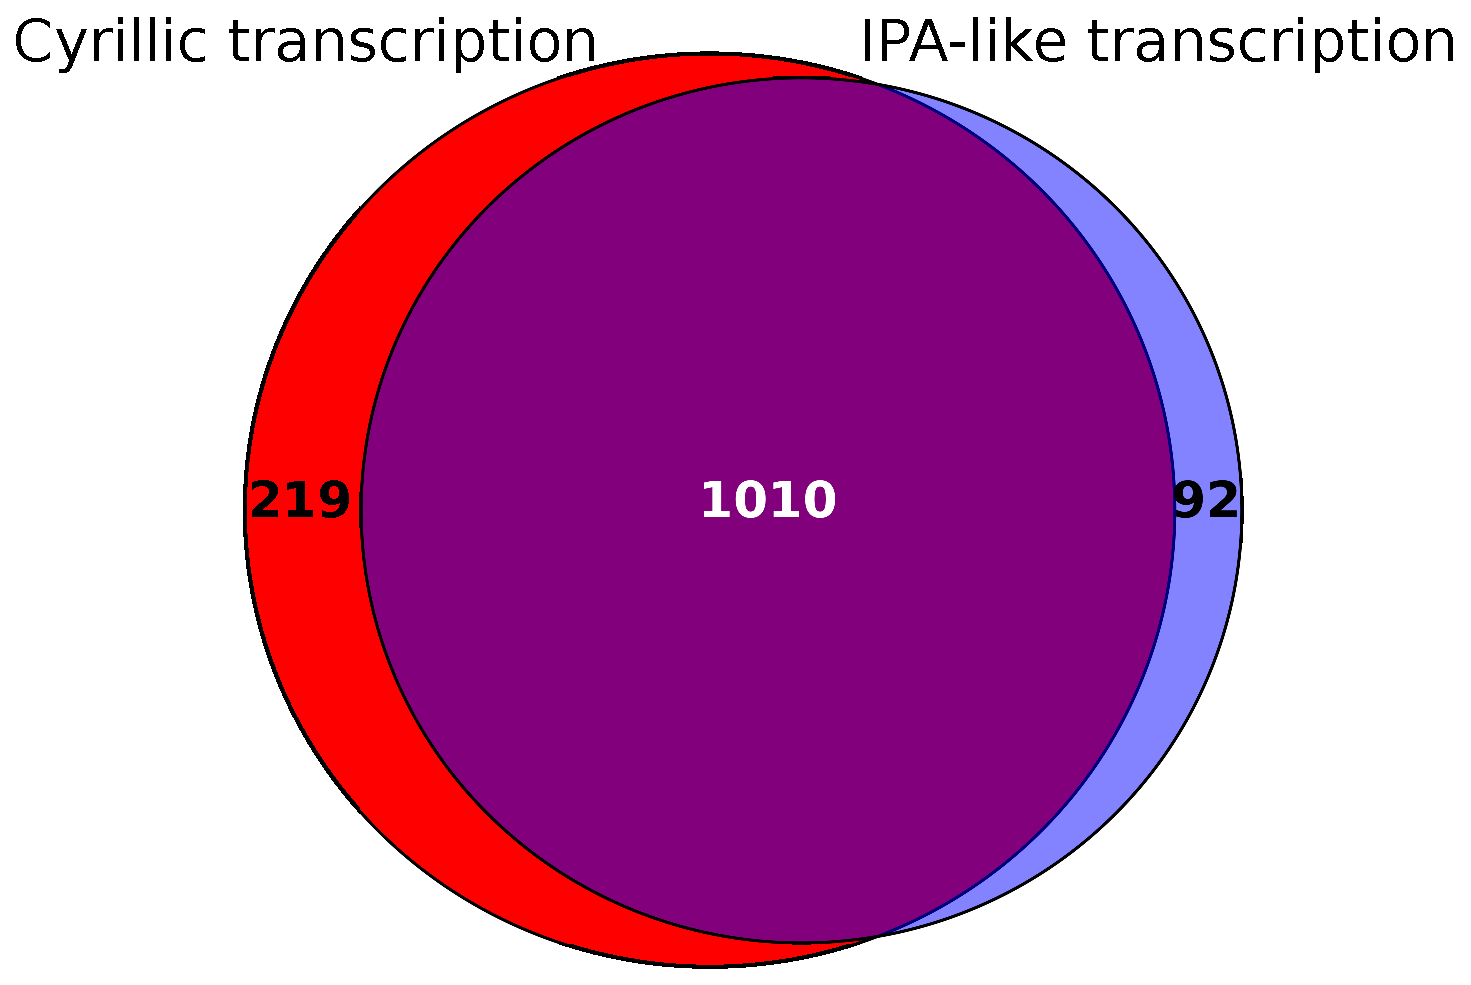
\includegraphics[width=0.45\textwidth,clip=]{figures/pairwiseVenn_sameMeaning}\\
      (a)&(b)\\
    \end{tabular}
  \end{center}
  \caption{Overlap between the pairwise cognates: (a) Pilag{\'a} and
    Mocov{\'\i} and Pilag{\'a} and the re-encoded wordlist of
    Mocov{\'\i}. 97.2\% of the cognate pairs are found in independently of
    the encoding. Reducing the FDR to 0.001, 97.5\% of the pairs are found
    independently of the encoding. (b) Tsez Mokok (IPA-like and cyrillic
    transcription) and Tsez Sagadin (cyrillic transcription). }
  \label{fig:encoding}
\end{figure} 

The second example was chosen to show that even drastic changes in the
encoding have only very moderate effects on the alignments and the
subsequent cognate identifications. To this end we use two different
transcriptions of the IDS wordlist of Tsez Mokok. One uses an IPA-like
transcription and the other one uses a cyrillic encoding. The wordlist were
obtained from different versions of the IDS. Thus we removed all entries
that are available in only one of the two transcriptions. Again, we
prepared two data sets, Tsez Mokok and Tsez Sagadin in cyrillic
transcription and Tsez Mokok in the IPA-like transcription and Tsez Sagadin
in cyrillic transcription. As for the artificial example, we trained a
bigram-model and used a permutation test to find a score-cutoff
corresponding to a FDR 10\% to produce a cognate judgements for both data
sets (see Fig.~\ref{fig:encoding}b). Most of the cognates were found
independently of the encoding (76\%). Using the same encoding, \ie{}
cyrillic transcription for both wordlists, yields additional 16\% cognates
that were missed when different encoding were used for the two
wordlists. For this experiment we used only one iteration to train our
bigram-model. The ability to detect cognates based on the alignment score
would likely increase when running multiple iterations. No attempt was made
to check whether the transcriptions are self-consistent, \ie{} whether
different signs were used to encode the same sound within a given
transcription. We also note the some noise in these data arises from
differences in the entries such as alternative suffixes or prefixes which
are sometimes provided within parentheses instead as an separate entry.
  
These experiments demonstrate that automated cognate detection is very
robust against small differences in the encoding used for the word list and
thus tolerates occasional errors in the data. In our \QUOTE{easy} example
we found a residual level of about 3\% discrepancies, which is small enough
to be tolerated in further analysis. Even for completely different encoding
schemes that follow different traditions we observe that the majority of
cognate call is independent of the encoding scheme. Substantially different
encodings, furthermore, mostly lead to a loss of sensitivity, \ie{} an
underprediction of cognates. In cases where the residual levels
discrepancies might be problematic, the automatically produced cognate
calls provide at least a very good starting point for further manual
curation of cognate assignments. And, of course, there is the possibility
to choose a smaller FDR value to obtain a smaller but more accurate set of
cognate pairs. Naturally, these claims are subject to regularities that are detectable at this level of representation, more likely to be found between languages with a relatively recent common history. Deeper genealogical relations are discussed on the basis of painstaking combinations of linguistic and historical knowledge, with little or no surface regularities on which contemporary methods could hinge on (e.g. \cite{robbeets2005})

\subsection{From non-parametric overviews to detailed probabilistic models.}

The approaches discussed so far were non-parametric. In the case of the
alignments, this in particular means that it was not necessary to include
prior knowledge about evolutionary process to obtain similarity measures
between words. There is no need to know how the languages are related to
each other, which proto-languages existed and what they looked like. This
becomes important if no clear model for the phylogeny is established yet,
the phylogeny could not be completely resolved, or the different models of
the phylogeny are still hotly debated. We, furthermore, showed that one
does not need to include the sound changes but can infer them indirectly
from the scoring model. The exact scores for matching the observed
characters can also be estimated based on the data. All these parameters,
namely the phylogeny and scores, would be defined \textit{a priori} in a
parametric method but do not need to \NEW{be} specified in the non-parametric case.

When applying the non-parametric approaches we discussed before, one needs
to choose the similarity measure that can be used to classify the related
languages. Since language change is a composite of many underlying
processes, the similarity measure almost always captures a composite of
many different pieces of evidence. For example, different words change at
different rates~\cite{Pagel:NatureLetter}, and consonants are perceptually
different from vowels in word recognition~\cite{Cutler:2000}.
\footnote{Again, we include changes in presence and absence of cognates as
  well as sound changes in the word \QUOTE{change}.} The most efficient use
of lexical data for determining deep language relationships, therefore,
should weight the stable words and consonantal identity more. 
\TODO{Is this a language independent result?}
The signal
from vowels is more informative when the vowel inventory is larger than
average.  In the non-parametric approaches, such choices of variously
weighting the evidence are choices external to the evidence, and made
\textit{a priori.}

In contrast, likelihood approaches depend on detailed models in which all
the parameters are simultaneously and consistently estimated. It can be
shown statistically that likelihood based estimation of models and their
parameters has many desirable asymptotic properties: in particular, they
automatically re-weight the data to answer each posed question
efficiently. In other words, the likelihood method \QUOTE{forgets} the
initial weighting of the data as the optimization progresses and reaches
the same end results irrespective of the the starting point. Consequently,
there is no need to choose a specific start point; instead any random
choice will do. These asymptotic properties, however, hold only if the
amount of data is large and the true generative model, \ie{} the true
evolutionary processes that lead to the observed languages and sounds, can
be well approximated by one or more of the models under consideration. Such
an approximation may take the form of ignoring the correlations introduced
by a set of complex unmodeled processes, replacing them with uncorrelated
random variables, or, instead, reducing the randomness by endogenously
specifying the correlations. As an illustration, consider the example of
modeling sound changes along the branches of the tree. Often sound changes
are conditioned, \eg{} they occur only in specific contexts. What if those
contexts are not known? We could simply model sound changes as rules that
are always applied if a specific sound occur. In this case we would
recognize that the model of unconditional sound changes cannot fit the
data. Let us assume, furthermore, we cannot model the unknown
context-dependencies since we do not have enough data to allow the model to
choose from all possible context-dependencies. The remedy in this scenario
is to ignore the context dependency and instead assume that a change occurs
only with a specific probability. Now we can fit the data. Even more, the
statistical procedure provides us with its best estimate to where a sound
change occurred and where it did not. Hence we can calculate the
correlations between the inferred sound changes with position, context, and
even with another sound change. In a refined model, one would condition the
probability of the sound change on these confounding factors.

The likelihood based models do not, in general, degrade gracefully as we
deviate from the condition that a tested model is an effective
approximation of reality. With vastly incomplete knowledge, therefore, the
choice between the likelihood based parametric approaches and the
non-parametric approaches described earlier is, essentially, a trade-off
between efficiency and robustness against model misspecifications, \ie{}
producing the correct results even though some aspects or parameter\NEW{s} of the
model are wrongly estimated.

Both classes of approaches---the parametric likelihood based models and the
non-parametric estimates based on similarity measures---ultimately rely on
a notion of \NEW{uniformitarianism}: that the process of language change and
diversification \NEW{does} not change over time. \NEW{Only}
in very heterogeneous, rapidly changing, or extremely long time
durations the \NEW{rates of this} process can be averaged over and approximated by
an additional uncorrelated noise. At intermediate times that is often the
most interesting, however, non-stationarity of the process is an important
problem. Non-stationarity in \NEW{these} cases usually means that the probability
distributions of sound changes change over time or that the scoring model
are different depending on the age of the words. Two partial solutions
ameliorate this somewhat. First, one can test the assumption of
uniformity~\cite{Hruschka:14} in the data set under consideration, so that
this and other modes of model failure can be quantified and incorporated in
the final confidence interval.\footnote{The confidence interval describe\NEW{s}
  the range of a parameter in which one expects the true value for this
  parameter to lie. For example, if we would know that there are
  differences in the rates with which sound changes happen, we could ignore
  the differences since they are very small. However, if we know about the
  size of the difference we could give the confidence interval for the
  results based on the size of the differences and observed data points.}
Second, models that allow a drift of the underlying process parameters,
such as rates of change~\cite{Thorne:98} or patterns of
covariation~\cite{Penny:01}, have been developed and used, and with enough
data, the extra parameters introduced can indeed be estimated.

\subsection{Computational methods and inference.}

Since computational methods today implement almost all of the traditional
methods of historical linguistic reconstruction, they have the large
potential to aid the traditional linguists in their research. The major
strength of computational methods is, however, the estimation of
approximate models from vast amounts of linguistic data. The output of such
a method is often presented as a properly scored choice between alternative
histories. For the likelihood-based approach of estimating Bayesian
posteriors, the final score can be interpreted as a measure of the rational
certainty arising from prior beliefs about model approximations and the
data at hand; such scores from various diverse evidence can, therefore,
often be combined to provide a composite picture without much additional
calculations.

These scores, moreover, are intended to formalize standard linguistic
understanding. The scoring method for a recently implemented likelihood
based method~\cite{Hruschka:14} can, for example, be described as proposing
sound correspondences, reconstructing intermediate ancestral forms
probabilistically and evaluating the ability of such a model to explain the
data with a minimum of extra random, \ie{} unexplained, changes. These
methods can be easily extended to simultaneously evaluate the proposed
intermediate sound systems and other features of the reconstruction, but
many rare processes are left out of models as a practical
consideration.\footnote{In a deeper analysis, the consideration is not only
  one of practicality but also of principle. Much of the purpose of
  quantitative methods is to demand a formal statement of the assumptions
  underlying a historical reconstruction. Ineffables, or evidence external
  to the data that can admit multiple interpretations, resist such
  formalization. Quantitative modeling forces the modeler to accept that if
  a few features cannot be explained without reference to a much more
  complex context than the evidence within the data itself, and if that
  context is ambiguous or subject to dispute, the model should adopt a
  least-biased assumption consistent with other assumptions that have been
  made in definite form as commitments of the model.}

Relative to this, the strength of manual curation lies in being able to
handle less data but many more particularized situations by inductively
drawing upon one's experience in various areas of linguistic, philological
and cultural knowledge that currently remain untapped by computational
methods~\cite{Starostin:10}. Though this approach suffers from the
well-known problem of over-fitting---seeing patterns in random noise---the
alternative of computational methods are only expected to be {correct on
  average.}  Individual nodes of a phylogenetic tree, reconstructions of
particular word forms, or determination of specific regular correspondences
can, always, be affected by model approximations. Even here, however, the
computational methods can be easily set up to \QUOTE{explain} its answers:
to provide, for example, not only a phylogenetic tree and the confidence we
ought to assign it, but also a list of evidence in favor of such a
reconstruction and conflicts that are left unresolved by the result. Such
evidence and conflicts, as well as a score indicating their significance
for the proposed reconstruction, can focus the attention of linguists and
guide further research.

While the methods sketched here complement and assist the labor of
traditional historical linguists, they constitute the only alternative
available in cases where information is scarce or contradictory. A
prominent case is that of the Tasmanian languages, discussed in detail in
\citet{Bowern:12a} (which we follow in the next paragraphs). After the
settlement of British settlers in the island (mostly during the 19$^{\rm
  th}$ century), native population experienced a sharp decrease in number
followed by what is usually perceived as a decomplexification process in
their material culture. 
\TODO{"After the settlement of British settlers in the island (...), 
native population experienced..."}\DB{This has been already fixed}
Little evidence about the cultural organization of
the Tasmanian people has survived, with different accounts differing in the
degree of unity or diversity across the island. 
\TODO{"...with different accounts differing in..."}
To worsen the situation,
few Paleolithic archeological sites exist, and the climatic conditions of
the island do not favor the conservation of artifacts. The genetic
information provides limited help since considerable European admixture
occurred after colonization. The linguistic evidence is not outstanding
either. There are a few wordlists (with a widely varying number of
elements) from all over the island, sometimes without precise information
about the location or any ethnographic or demographic information about the
speakers that served as informants. Based on this data, researchers have
argued about the unity or diversity of Tasmanian languages, with perhaps
the most widely accepted opinion being that linguistic analysis can lead at
most to rejecting the idea that Tasmanian languages constitute a single
linguistic family \cite{Crowley:1981}.

By using a combination of methods from evolutionary biology---prominently,
phylogenetic inference---Bowern was able to gather enough evidence for 4/5
groupings (tentatively referred as macro-families) present in the wordlists
that correspond somewhat with earlier archaeological classifications, while
at the same time lending support to the idea that Tasmanian languages are
not all directly related, at least to the time depth accessible to the
methods and the data. Not only did the usage of methods from evolutionary
biology allow Bowern to determine the number and extension of putative
genealogical groups among the Tasmanian languages, but, more importantly,
the usage of those methods lead to a natural quantification of
uncertainty---so, for instance, while the evidence for a common ancestry of
two of the inferred groups (those from Bruny Island and Oyster Bay) is
strong, the estimate of the common root age is extremely imprecise, ranging
from anywhere from 2,000 ybp to 20,000 ybp or more.

\subsection{Putting dates on language trees.}

One important aspect of statistical modeling is that different aspects of
the result have different confidence intervals and even different
requirements on the underlying model. This is as true for computational
methods as it is true of manually derived phylogenies: one often attributes
a much higher certainty to the identity of the various large sub-families
of Indo-European than to their relationships to each other. In
computational linguistics, one piece of the result---the absolute dates of
various events---is often more uncertain and controversial than the
classification. This mimics similar controversies that have arisen in
molecular dating of the origin of biological taxa. The reconstruction of
the phylogenetic tree, specifically its topology, requires only that the
underlying process conforms to a so-called additive tree, \ie{} branch
lengths measure the total amount of change that has occurred along
them~\cite{Semple:03}. As a consequence, a large array of rate variations
occurring independently along the different branches of the tree do not
affect our ability to correctly reconstruct them. Dating, on the other
hand, requires an explicit clock and hence a way to explicitly model rate
variations so that an ultra-metric tree can fit to the data.
 
Dating in phylolinguistics is a complex subject where methodological
consensus has not been reached yet~\cite{Heggarty:06}. Ultimately, since
dates rely both on linguistic and non-linguistic evidence, this is not
entirely unexpected. To convert the relative divergence times of the
various branches to absolute times, information for some of the splits has
to be in-built into the prior structure, which later permits to infer dates
(and rates) along with branch lengths~\cite{Gray:11}. For
instance,~\citet{Gray:03} fixed the ranges of coalescence of most of the
Indo-European sub-families based mostly on historical records from the
Roman Empire and Medieval Europe period, and in~\citet{Gray:09} they
studied the expansion of the Austronesian family while constraining the age
of some of its sub-families on evidence from archeology.

To obtain the dates of unknown events from the dates of a few known events
\NEW{requires} a model about the rates of change; equally, however, the known dates
allow one to evaluate any assumption one makes about them. The original
proposal of glottochronology was to assume that the number of cognate
retentions of two languages diverging at a given time decays exponentially
with constant rate~\cite{Swadesh:55}---which is analogous to the strict
molecular clock hypothesis in molecular evolution. Rate regularity has been
severely criticized since early on~\cite{Bergsland:62, Blust:00}, although some
support for the idea still exists in other
contexts~\cite{Ehret:00,Starostin:00,Starostin:13,Holman:11}. 
\TODO{None of these paper support the idea of rate constancy, they support
(emprirically) the idea of rate regularity.}\DB{change constancy for regularity}
Within the
context of a likelihood based approach, the regularity of the rates
of various features can be tested~\cite{Hruschka:14}, as can particular
hypotheses about factors affecting changes in the different
branches~\cite{Pagel_rates}.

A natural extension of this idea is to allow individual pairs of languages
or whole branches to have their own independent rates
\cite{Embleton:86}. Such an unconstrained model, however, introduces too
many degrees of freedom, which leads immediately to estimated parameters
with large variance. A widespread solution to this conundrum is the
application of some kind of regularization constraint on the different
rates, in such a way that large variation of rates within lineages is
penalized~\cite{Sanderson:02}, though alternate statistical methods that
fix the probability distribution of the rates, rather than the rates
themselves, can be easily implemented in a Bayesian framework
\cite{Korber:00}. Again, to the extent that the data does not contradict
them, simple approximate models involving rate constancy, but allowing
unmodeled sources of dispersion, are expected to outperform more realistic,
but complicated models, in terms of providing valid estimates with
defensible error bands. With respect to the actual processes used to model
cognate loss and retention, researchers, therefore, usually adopt simple
parametric models taken from evolutionary biology~\cite{Nichols:08},
although some more realistic alternatives have been developed as
well~\cite{Nicholls:06,Starostin}. Even when such approaches fail to answer
the methodological question of how reliable molecular clocks are expected
to be in a given situation, they do allow one to come up with more
realistic confidence intervals for the inferred dates.

\section{Models of meaning.} 

\TODO{It is never declared how synonyms are treated in the IDS and in the
experiments of Section 4 and how prevalent that is.}

Discussion of lexical connections between different languages often suffer
from the fact that the meanings expressed by these lexical items have not
yet been formalized. A word meaning covers a region of a multidimensional
conceptual space; it is difficult if not impossible to identify discrete
word senses~\cite{Croft:04, Koptjevskaja-Tamm:08}. Semanticists ideally use
stimuli representing particular situation types (images, video,
questionnaire sentences) to elicit a range of points in the conceptual
space~\cite[e.g.][]{Berlin:69, Dahl:85, Levinson:03, Majid:08,
  Croft:08}. However, historical linguists rarely if ever do so, in part
because they frequently must rely on secondary sources and documents from
extinct languages for comparison. Although historical linguists recognize
the problems of discrete word senses in considering lexical reconstruction,
in applying the comparative method they implicitly assume a model of
discrete word meanings or at least of semantic overlap across the words in
languages to be compared~\cite{Fox:95}. In effect, English (or another
language used by the historical linguist) functions as the semantic
metalanguage for comparison of word meanings. Word meanings also overlap
with other word meanings in a language, and shift both gradually (e.g.
extension and retreat in a semantic domain) and discontinuously, via
processes such as metaphor and metonymy~\cite{Sweetser:90, Traugott:02};
and little cross-linguistic research has been done on the likelihood of
various types of semantic shift, except in restricted domains such as body
part terminology~\cite{Brown:76, Brown:79, Witkowski:78, Wilkins:96},
cardinal directions~\cite{Brown:83}, perception verbs~\cite{Viberg:83},
concepts associated with fire~\cite{Evans:92}, and color
metaphors~\cite{Derrig:78}. As a result, outside a very restricted domain,
comparison of words to obtain cognates is often done primarily based on the
validity of regular sound correspondence with little weight on semantic
content~\cite{Nichols:96}. A complete probabilistic model for inferring
language relationships, however, needs to include probabilistic aspects of
meaning correspondences as well.

\subsection{Paralogous words.} 

This element of cognacy across meaning category is analogous to an
important mode of biological evolution---the duplication and subsequent
functional divergence of genes. Indeed, a large fraction of the protein
inventory of most organisms has arisen in this manner. It is largely
unknown whether a similar mechanism is at work in human languages, \ie{} to
what extent a given language harbors cognate words with different
meanings. English language examples of such \TT{paralogous cognates}
\emph{tell/\penalty0\hspace{0pt}talk}, \emph{lay/\penalty0\hspace{0pt}lie},
and \emph{raise/\penalty0\hspace{0pt}rise} demonstrate that such word pairs
exist.\footnote{We ignore for this discussion examples like
  \emph{spring(verb)/\penalty0\hspace{0pt}%
    spring(season)/\penalty0\hspace{0pt}spring(source)/\penalty0%
    \hspace{0pt}spring(coil)} where the identity of form allows us to treat
  them either as paralogs or as semantic extension from a single sense.}
The loss of ancestral morphological forms together with the retention of
\TT{frozen} word forms as \TT{new} words provides a mechanistic explanation
for such examples. Again we will, for the sake of this contribution, not
pursue the issue of possible mechanisms. Instead we ask here a much simpler
question: Is there evidence for \TT{paralogous words} as a wide-spread
phenomenon?  In other words: do data \NEW{sources} accessible to us contain
sufficient information and signal to start investigating paralogous words
in a systematic manner? For the purpose of this position paper we will
demonstrate how these questions can be addressed by means of a suitable
statistical approach. We will leave a more detailed analysis of the topic,
which is ongoing work, for a subsequent publication.

We have to make one single assumption about paralogous cognates, namely
that they inherit both their phonological form and their meaning from a
common ancestor. Conversely, we assume that a simultaneous similarity of
meaning and phonological form, if not explanable by chance, can result only
from paralogous cognates: 
\TODO{As it is written this is two assumptions. Actually the first is
the definition of paralogous and what you assume is the second
one (that only paralogous cognates have sim in form and meaning).}
\ie{} processes like sound symbolism are
sufficiently weak that they can be ignored for this purpose. If paralogous
cognates exist, they will therefore be recognizable in the data as similar
words that also fall into the same broad semantic groups of meanings. We
have already seen above how phonological forms can be compared in the
context of computational cognate detection. We will adapt this approach to
become applicable to words from the same language. The comparison of
meanings is conceptually more difficult. However, we do not need a detailed
theory or representation of meaning. For our purposes it is sufficient to
be able to decide whether some word pairs are semantically closer than
others. We can therefore make use of the semantic classification of the
words in word list data. As discussed above, the IDS data~\cite{IDS} are
grouped into \QUOTE{chapters} that correspond to very broad semantic
categories. We can therefore structure our analysis in the following
manner: If two similar words are completely unrelated and accidental, then
they will appear at random places in \NEW{the} word list\NEW{s}. On the other hand,
paralogous cognates will retain some semantic similarity and hence
predominantly appear within the same chapter of the IDS word list. It is
important to recall that our purpose is to check whether there is evidence
for paralogous cognates in the first place, not to understand them in full
detail. We therefore devise a simple test for the association of similar
words with similar meanings: we simply ask whether there are more pairs of
similar words within a chapter than between chapters, and if so, whether
the difference is statistically significant.

To do this in practice, we compare for each language two samples of 1000
pairs of non-identical words. We remove identical words with different
meanings since we only interested in paralogs, \ie{} words that are
distinct, not in words that have simply expanded their semantic scope. 
\TODO{The removal of identical words is contrary to the stated interest
which was "This element of cognacy across meaning category is
analogous to an important mode of biological evolution—the duplication
and subsequent functional divergence of genes.". Surely identical
words are (always or sometimes) instances of this process. For example,
mouse is an animal and now also a computer device, with its own life
in the different senses (e.g., the computer device can have a different
plural).}
The
first sample comprises word pairs from the same chapter. In the second
sample we only include word pairs from two different chapters. Then we
determine, separately for each sample, the number of word pairs that are
phonologically similar using the same alignment scores that we have
employed already for cognate detection in section~\ref{Sect:SimReg}. More
precisely, we consider two words $x$ and $y$ from the same language $A$ as
similar if $score(x,y)>\theta(A)$, \ie{} if their similarity is larger than
a language-specific threshold $\theta(A)$. This threshold value is also
estimated from the word list data in complete analogy to the thresholds
used earlier for cognate detection. Again, the bimodal form of the
distribution of the scores of all word pairs for language $A$ is the key,
and we remove languages from this study when the bimodality is not obvious
\NEW{, \ie{} there is only little data for these languages}
(see Fig.~\ref{fig:cutoffChoice}). Our pairs of similar words therefore
have the same statistical characteristics as cognates, except that they are
taken from the same language, and may not correspond in meaning too
closely.
		
\begin{figure}
\begin{center}
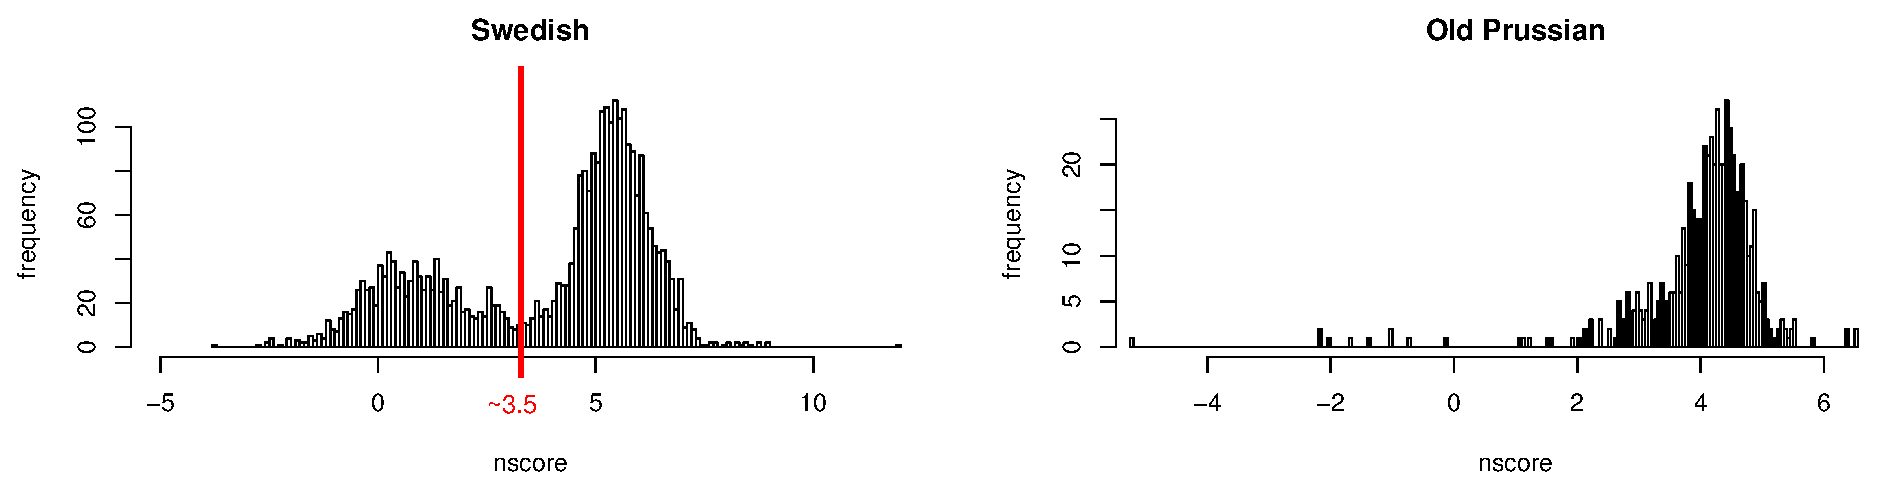
\includegraphics[width=0.9\textwidth]{figures/cutoff}
\end{center}
\caption{Distribution of normalized alignment scores for (left)
  Swedish and (right) Old Prussian. For alignment scores of Swedish
  words, a bimodal curve can be seen. The left hill is assumed to
  represent scores of unrelated words, while the right one mostly contains
  alignments of similar words. Therefore, the cutoff is set to $3.5$ as
  this score separates the two hills. The distribution of
  alignment scores in Old Prussian shows that the data here is rather
  sparse. Hence, no cutoff can be chosen and the dataset was removed from
  this experiment.}
\label{fig:cutoffChoice}
\end{figure}
	
The results of this sampling procedure are two numbers $n_s$ and $n_d$ for
each language $A$: the number $n_s$ of pairs of phonologically similar
words among 1000 word pairs from the same chapter, and the number $n_d$ of
pairs of phonologically similar words among 1000 words from different IDS
chapters. For each language, the parameter \(\delta = (n_s-n_d)/1000\)
therefore measures (as a fraction of all word pairs) the excess of similar
words with similar meanings over similar words with unrelated meanings. A
positive $\delta$-value consequently indicates that a language contains
more non-identical words with similar meanings than expected. For a single
language we might observe a positive $\delta$-value by chance. In
Fig.~\ref{fig:deltas}, we therefore plot the frequency distribution of the
$\delta$-values for large language groups, including Indo-European and
Caucasian languages, as well as for a sample of 155 languages from the
IDS. If similar, non-identical words do not systematically have similar
meanings we expect that this distribution is centered around zero.

\begin{figure}
\begin{center}
\includegraphics[width=0.45\textwidth,clip=]{figures/deltaplot}
\end{center}
\caption{Distribution of $\delta$ in Indo-European, Northern-Caucasian, and
  all other languages (see Table~\ref{tab:langDeltas}). Medians of the
  distributions are shown as filled circles. We did not observe
  $\delta$-values smaller than zero. If there would not be a signal, the
  $\delta$-value would distributed symmetrically around zero as, for
  example, in Fig.~\ref{fig:Chist}.}
\label{fig:deltas}
\end{figure}

We find, however, that for all languages $\delta>0$, even though the values
are close to $0$ for some languages (Fig.~\ref{fig:deltas}). This is
extremely unlikely if the values are drawn from any distribution centered
about zero. In fact, the probability that 155 independent numbers from such
a distribution all end up with the same sign by chance is less than
$10^{-46}$. This indicates that there is indeed an an association between
similarity in meaning and similarity in the form of the words. The
distribution of $\delta$ for language groups shows medians around
$\delta=0.014$ providing an estimate for the fraction of words that have a
similar copy with similar meaning. This simple analysis indicates that word
paralogy is a pervasive phenomenon across essentially all language groups
that deserves a more detailed investigation in the future since
\NEW{all} language\NEW{s} have a $\delta$-value larger than zero.

\subsection{Polysemy.} 

The concept of paralogous words is closely connected to the idea of
polysemy: words acquire additional meanings with continued use, often
due to culturally salient metaphors or widely used metonymies.
Individual instances of these are extremely historically contingent, but
the universal features that make languages useful and learnable are
expected to be reflected in the statistical patterns of these changes. The
signatures of such patterned changes should, therefore, be visible in the
patterns of polysemy across the world's languages.

\begin{figure}
\begin{center}
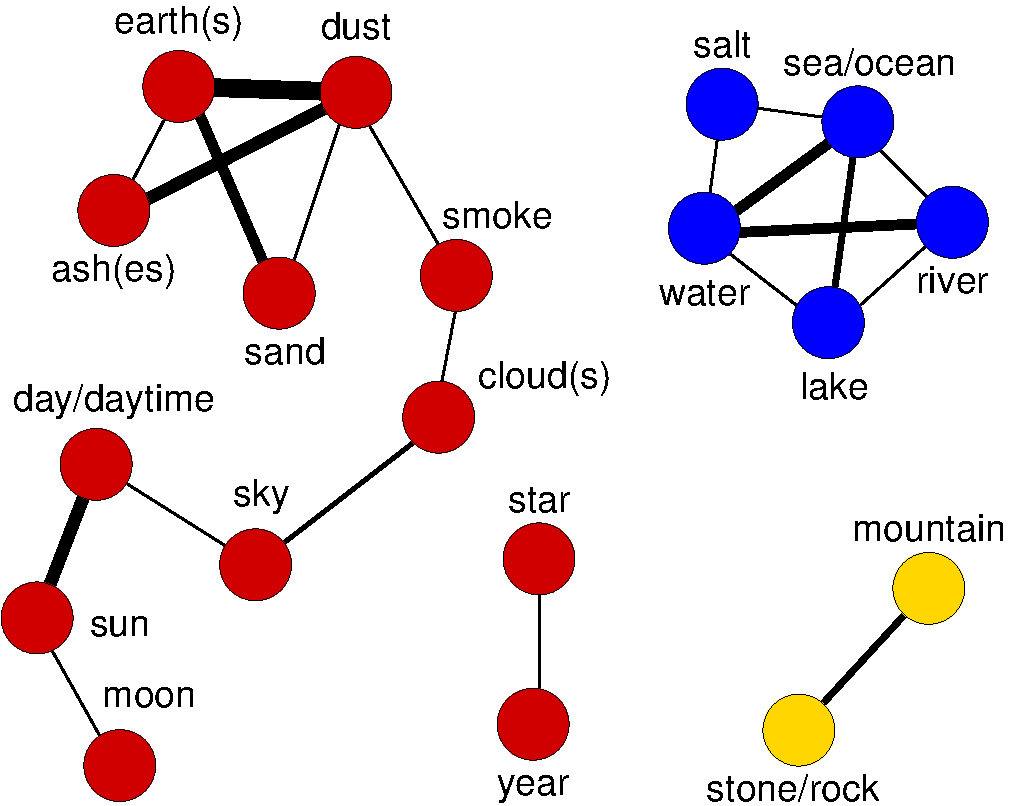
\includegraphics[width=0.5\textwidth]{figures/cg_swad}
\end{center}
\caption{A portion of the lexical semantic network presented in
  \citet{Youn:16} showing the heterogeneous connectivity structure of the
  lexical semantic network. The nodes are Swadesh concepts linked if there
  exist languages with words polysemous between the two concepts. The links
  are weighted proportional to the number of such polysemies, and rare
  single polysemies are omitted for simplicity. The data are collected from
  bilingual dictionaries of eighty-one languages unrelated at the level of
  genus in the standard linguistic classification. As clearly shown in the
  diagram, some concepts like \QUOTE{water} or \QUOTE{earth} are involved
  in many polysemies, whereas others like \QUOTE{moon} in very few. Further
  analysis reveals that these concept form three almost disconnected
  clusters shown here using different colors.}
\label{fig:semanticnet}
\end{figure}

A recent work~\cite{Youn:16} provides a quantitative assessment \NEW{of} the
patterns of polysemy using cross-linguistic dictionaries. When a word in a
meta-language is translated to a language of interest, additional meanings
may appear if the word is polysemous in the language. The study builds a
collection of cross-linguistic polysemies for a few concepts chosen from
Swadesh list across a set of languages sampled to be representative of
worldwide diversity. Then, a semantic network is constructed for each
language where nodes denoting concepts are linked if they are represented
by a polysemy. \NEW{Fig.}~\ref{fig:semanticnet} shows an aggregated network
obtained from the entire set of languages. A randomization test showed that
the polysemy relations were statistically universal across the
languages---the network of relationships captured by any random subset of
languages \NEW{was} significantly correlated with that obtained from the
complementary subset, but different from what one would expect merely from
the amount of polysemy observed for the different words. With further work,
this should be translated into an empirical prior on the capacity of
different meanings to be expressed by the same word.

\begin{figure}
\begin{center}
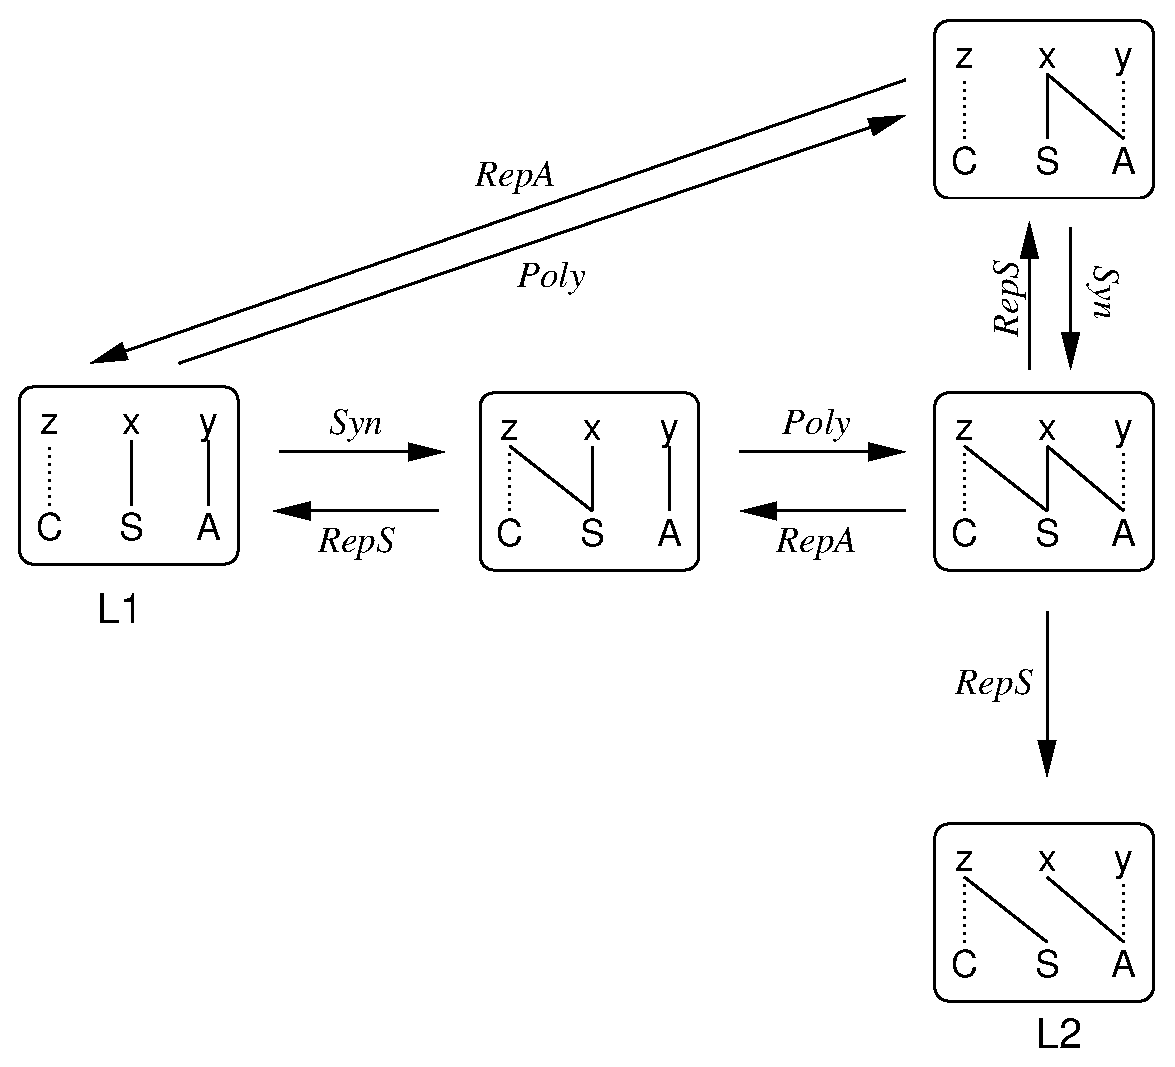
\includegraphics[width=0.65\textwidth]{figures/SPM}
\end{center}
\caption{A model of how semantic shift takes place through intermediate
  polysemy and synonymy. Meanings, represented here by capital letters, are
  expressed by words represented by lowercase letters. Over time,
  polysemies (a word representing more than one meaning) and synonymies (a
  meaning represented by more than one word) are generated by additional
  word-meaning links being generated, whereas loss of word-meaning links
  leads to loss of polysemies and synonymies. The net result is often a
  word replacement in which a word with one meaning can shift to being used
  to express a different meaning. In the figure, the word-meaning
  associations that may be the focus of a study are depicted by solid
  lines, whereas dotted lines represent associations outside the study set
  that may not be directly observed. The possible paths arising from sense
  extension are labeled as \textit{Poly} indicating development of a
  polysemy or \textit{Syn} indicating development of a synonymy, and sense
  specialization leading to a word losing the sense \textit{X} is indicated
  by \textit{RepX}.}
\label{fig:state_process_model}
\end{figure}

When words change meanings, the process involves a number of intermediate
steps as illustrated in Fig.~\ref{fig:state_process_model}. The
intermediates involve the diversification of meanings of words leading to
polysemies, and the meanings of different words overlapping, leading to
synonymies. In addition, novel words arise by morphological processes or
adoption of foreign words, and word senses get specialized by the loss of
rarely used meanings especially when large clusters of synonyms exist. The
detailed parameterization of this state process model has not yet started,
but databases of attested meaning changes across the language families of
the world are being assembled~\cite{Zalizniak}. Careful study of polysemies
and typologically frequent, or \QUOTE{trivial}, semantic shifts is of
particularly vital importance to hypotheses of distant phylogenetic
relationship, since the quantity of direct semantic matches between
languages declines progressively, depending on the time distance that
separates them. Some steps in that direction are currently being taken by
members of the EHL program~\cite{EHL}, working on algorithms for automated
comparison between expanded word-lists consisting of a fixed 400--500
elements, as compared to Swadesh's original 100--200. These algorithms take
into account the possibility of \QUOTE{trivial} semantic shifts, based on a
preset listing of such shifts that is being extracted from polysemies and
indisputable low-level semantic change, elicited within the
comparative-historical databases created by various members of the program.
\TODO{I cannot find any information on the EHL website cited here 
on the work being done there on semantic shift. If it is not possible
to cite outcomes of that work it may be preferable to omit the 
discussion of that work in progress.} \NR{Ich kann es auch nicht finden.}

\section{Measuring the success of statistical methods.}

\NEW{In the previous sections w}e described several statistical \NEW{methods} and
discussed their application\NEW{s to} different aspects of language evolution.  We
demonstrated in \NEW{the} sample application that the results are reasonable.  One
might argue, however, that we chose \QUOTE{simple} cases where the answer
is already known. This may not immediately convince the reader that the
methods will also work in \QUOTE{hard} cases, where the signal is weak and
multiple hypotheses are still debated in the linguistic community. Thus,
the question is how to prove that a method provides useful and reliable
results in the hard cases? The problem of assessing the reliability of a
method or a specific software tool has been well studied in the context of
computational biology. In this section, we sketch these methods of
verification with examples relevant to historical linguistics.

Statistics provides \NEW{a} measure for the confidence in the results produced by a
computational method. Throughout this \NEW{contribution} we have used three of
these measures: specificity, sensitivity, and the FDR (see
Figs.~\ref{fig:DanROC} and \ref{fig:FDR}). Sensitivity and specificity are
calculated with respect to a known ground truth, often called the
\QUOTE{gold standard}. It is common practice therefore, to test methods on
well understood examples.

A good method has two features: (1) it works successfully on
\QUOTE{perfect} data, and (2) the results are robust against noise and
errors of the kind that can be expected to be present in the input data. In
computational biology, the robustness is often tested using simulated
data. We have used the same idea above to test the robustness of cognate
identification with respect to errors and differences in the encoding of
word list data. The artificial data sets can be used to benchmark methods
and to estimate their error rates. Since the noise is modeled explicitly,
conclusions on the robustness of the method towards different noise can be
estimated.

Such simulations, however, require a knowledge of the underlying processes
to produce representative data. In cases where we know little of the
underlying processes, we need to use a different approach. A particularly
interesting method is called \TT{cross-validation}. It consists of modeling
the behavior using a subset of data and testing it out with the other
subset. Even when one is unable to test the results on a left out set, the
variation in the results as different random subsets are analyzed can be
used to estimate the uncertainty inherent in the method.

As an example, imagine one would like to evaluate how good the likelihood
method works but there is no model of evolution of sound systems and
cognates that reproduces faithfully all relevant features expected in the
data. If one has enough cognates, one can apply the leave-out
approach. This consists of running the analysis method on sub-samples of
the observed data. A robust method will show almost the same results for
any large sub-sample. Furthermore, the result from any such sub-sample will
agree with the result obtained from the whole data set. For example, the
likelihood method described above results in a phylogeny with sound changes
assigned to the branches. One therefore tests whether the phylogeny and the
predicted sound changes are essentially independent of the
sub-samples. Similarly, the correctness of the scoring model can be tested
with this approach by training the model with sub-samples of the data. The
test can be made more quantitative by observing that statistics can often
predict how the uncertainty in estimation resulting from sampling biases
and variances changes with sample size, and tests with sub-samples of
various sizes can verify these predictions.

\section{Conclusion.} 

\TODO{The conclusion contains information not in the body of the paper and
should thus be reorganized.}

Biological and language data share enough properties to argue that methods
developed in one domain are also applicable in the other. Comparative
methods are useful in both fields as a means to infer the evolution of
species or history of languages. Words as well as genes, proteins, or RNAs
are encoded in a linear manner, and their \NEW{comparison} is usually based on
alignments. In biology, it is possible to formulate explicit models with
just a few parameters that have to be estimated. The amino acids and bases
at alignment positions change almost independently and thus almost
identical models can be applied to all domains of life. This is not the
case for linguistics, where the fundamental processes of evolution are not
yet properly understood and modeled. This, however, merely cautions against
the uncritical use of molecular phylogenetics programs directly for
linguistics: not against reimplementing the tools and methods that have
been specifically developed to discover the regularities from the
linguistic data themselves. Furthermore, permutation tests, as shown in
this paper, are model independent. They allow tests of phylolinguistic
hypotheses even in the complete absence of mechanistic or detailed
statistical models.

In our presentation above we have highlighted but a few aspects of
  language evolution. There are, of course, numerous others. Grammatical
  features, for example, are subject to evolutionary turnover as well.  The
  work of \citet{Dunn:11} highlights an important issue\NEW{,} on the one hand,
  features of language may well be correlated. On the other hand, most
  regularities are of a statistical nature rather than absolute
  ``universals''. Phylogenetic relatedness naturally introduces such
  correlations. It becomes an important issue, then, to disentangle
  regularities in language evolution that are grounded in cognitive,
  physical, or biological constraints from those that are a mere reflexion
  of lineage-specific persistence. As a case in point, some of us recently
  revisted \cite{Blasi:16a} the presumed independence of sound and meaning,
  which is widely believed to be a crucial property of human
  language. Surprisingly, a careful statistical examination of words from
  nearly two-thirds of the world's languages reveals that unrelated
  languages very often use (or avoid) the same sounds for specific
  referents. This effect cannot by explained by phylogenetic relatedness or
  geographic proximity but emerge independently. At present we cannot give
  a mechanistic explanation for most of the statistically signficant
  sound-meaning associations---but we could quite easily incorporate them
  into the background statistics used, e.g., for cognate detection,
  with the effect of increasing sensitivity.

Computational linguistics methods have the potential to carry out all the
major steps of historical reconstruction starting with lexical data,
especially when curated manually with detailed linguistic knowledge to
separate the roots from the affixes. These methods can be used to determine
when sound similarity is high enough to merit a closer
scrutiny~\cite{Turchin:2010}, to infer regular sound
correspondences~\cite{Hruschka:14} and
cognates~\cite{Frunza:08,Kondrak:09,Hall:11,Steiner:11a,rama2013two}, to
take phonetic context into account and reconstruct ancestral
forms~\cite{BouchardCote:13}, and to use these---as well as cognate
loss~\cite{Gray:00,Gray:03,Pagel:NatureLetter}---to classify language
families and arrange them into a phylogeny~\cite{Hruschka:14}. These
methods infer and incorporate limited amounts of rate variation across the
various lexical items and lineages, and provide a quantitative evaluation
of various hypothesis, often in probabilistic terms that can be translated
across different data domains. Even though these methods do not currently
incorporate rare phonetic processes like metathesis and analogical change,
nor do they evaluate the reasonableness of the phonetic system in their
inferences, such additional processes and constraints are reasonably
straightforward to add in when and where they become important. 
\TODO{Though analogical change is sometimes treated as a "garbage 
bin" of marginal, non-regular changes, the phenomenon is really
not that rare (certainly not in the same class of unusual "phonetic 
processes" as metathesis, though of course metathesis can happen by 
analogy...). Non-regular does not mean rare. Nor is it the case that 
analogical changes are inherently non-regular. It's a little unclear,
therefore, exactly what you are trying to single out here as being 
poorly handled by these methods.}
The
required parameters can again be learned based on the data. As long as the
effect of each particular language contact on the lexicon is reasonably
small, methods from biological phylogenetics~\cite{Griffiths:97,Arenas:13}
can be used to factor them into the inference. More problematic is
quantifying whether a reconstructed lexicon is reasonable. Work on
quantifying lexical semantics, however, holds promise for modeling semantic
shift, thus providing an avenue to approach this problem systematically.

It is important to highlight that the task of a statistical inference
algorithm is never to parameterize the most complete and complex known
model based on the data. Rather, it is to resolve the model into those
parts that affect multiple independent pieces of data so that the
correlations between them can be used to properly parameterize the model.
Those processes that affect only a small number of independent facets of
the data ought to be modeled as \TT{random effects} since the data
constrains the total strength and structure of the combined effects of all
such processes far more than it constrains the correlation produced by any
one of them. As the amount of available data increases, or our
understanding of such processes increases, they can be added back, possibly
under the control of priors that incorporate our independent knowledge of
their strength and structure.

The major goals of quantitative modeling may be encapsulated in a few
points. Each of these depends, in one way or another, on the ability of
algorithms and high-performance computation to carry out sorting and
tracking tasks at which computers are strong and humans are weak. The first
is that quantitative models may simultaneously retain a large variety of
hypotheses about history, and assign scores to them that result from
explicitly stated criteria, consistently imposed. The second is that
probabilistic methods may weigh joint evidence of relatedness from
intermittently-preserved features in languages. While any single feature
may be unreliable and carry limited information, the number of
incompletely-preserved signatures of relatedness may be sufficiently larger
than the number of strong signatures, that the weak signatures in aggregate
provide a large or even leading part of the information available in the
data. This is analogous to fingerprinting, in which both single features
and the comparison of global parallels enable the assignment of
similarity. The third is that formal models require the modeler to be
explicit about premises, and provide systematic commitments to what it
means to minimize bias over evidence that cannot be crisply
formalized. This does not require the elimination of context or ambiguous
premises; rather, it incorporates these in priors, so that the modeler asks
\QUOTE{what weight of evidence would be required to convince me that my
  prior premise was incorrect?}  Fourth, quantitative methods permit
efficient backtracking if results are obtained that conflict among methods,
or that conflict with trusted knowledge from outside the linguistic
problem. Backtracking means isolating the key assumptions on which
differing conclusions depend, either enabling a study of the relative
strength of differing positions, or signaling the kinds of
currently-unavailable data that would best resolve them. Fifth,
quantitative methods, simply by showing what can (and what cannot) be
reliably computed from given assumptions and evidence, can expose different
frames for questioning or different concepts for interpretation, which
might have remained hidden from the perspective only of manual
reconstruction. Sixth, even in the \QUOTE{hard} cases where signals are
weak or multiple signals overlayed, computational methods can come in
handy. Computational methods do not simply return whether a hypothesis is
true or not but rather how likely they are. Thus, when data \NEW{are} noisy,
different hypotheses can be tested and unlikely hypotheses can be
discarded. Discordant results from application of different methods may
point to hypotheses resolving the apparently incoherent array of
conclusions.

Formal methods never replace human thought, and the subset of premises and
evidence that can be expressed formally is always incomplete within the
domain available to human expertise. We should recognize, however, that the
unaided human mind was never the widest possible window through which to
experience the world. New devices for measuring, organizing, and computing
have enlarged the power and also the conceptual scope of human thinking in
all of the natural sciences, often in unanticipated ways. The promise of
computational methods to historical linguistics is likewise to allow minds
to see the language world in all their existing capacities, and in new
capacities as well.

What these methods, then, allow one to do is to take the tedium out of the
work of linguistic reconstruction. The computational codes are not designed
to supersede the knowledge and efforts of the careful historians and
linguists: rather, its primary use, at least initially, ought to be in
helping evaluating hypothesis. It is reasonably straightforward for these
computational methods to output not only a scored list of alternative
hypotheses, but also a scored list of evidence that supports and refutes
any hypothesis. This can focus the valuable time of researchers in
understanding and weighting the contradictions. This then is the division
of labor that one can envisage: linguistic knowledge alone prescribes
\NEW{what questions are interesting and what constitutes adequate
  support for or against them---how this is done is what the focus on
  computational linguistics should be.}

\clearpage
%
\section*{Appendix a: bigram alignment algorithm.} 
\phantomsection\addcontentsline{toc}{section}{Appendix a: bigram
  alignment algorithm}
\label{AppA}

Word alignment\NEW{s} are performed with an extension of Needleman-Wunsch
algorithm \cite{needleman:70} that computes optimal alignment for linear
gap cost models such as the Levenshtein distance \cite{Levenshtein:66}. The
linear gap model is not ideal, however. Instead, it is desirable to
penalize longer gaps subadditively. The simplest such model \NEW{uses} affine gap
costs, in which the opening of gap incurs higher costs than gap
extensions. An efficient dynamic programming algorithm for this version of
the problem was given by \citet{Gotoh:82}. In order to accommodate
overlapping bigrams as the basis of the scoring model we further modify
this method.

Consider two words $X = x_1\cdots x_n$ (from language $P$) and $Y = y_1
\cdots y_m$ (from language $Q$) of length $n$ and $m$. Denote by $M_{i,j}$,
$D_{i,j}$, and $F_{i,j}$ the score of the best possible alignment of the
prefixes $X = x_1\cdots x_i$ and $Y = y_1 \cdots y_j$ subject to the
constraint that alignment ends in a match or mismatch, in a gap in the
first sequence $X$, and in a gap in the second sequence $Y$, respectively.
These scores must satisfy the recursions
\begin{equation}
  \begin{aligned}
    M_{i,j} &= \max  \begin{cases} 
      M_{i-1,j-1} + \sigma(x_{i-1}x_i,y_{j-1}y_j),\\
      D_{i-2,j-2} + \sigma(x_{i-1}x_i,y_{j-1}y_j),\\
      F_{i-2,j-2} + \sigma(x_{i-1}x_i,y_{j-1}y_j)\}
                 \end{cases}
      \\
    D_{i,j} &= \max  \begin{cases} 
      M_{i-1,j} - \Delta_{PQ}(x_i),\\
      D_{i-1,j} - \delta_{PQ}(x_i),\\
      F_{i-1,j} - \Delta_{PQ}(x_i)\}
                     \end{cases}
      \\
    F_{i,j} &= \max \begin{cases} 
      M_{i,j-1} - \Delta_{QP}(y_j),\\
      D_{i,j-1} - \Delta_{QP}(y_j),\\
      F_{i,j-1} - \delta_{QP}(y_j)\}
                    \end{cases}
  \end{aligned}
\end{equation}
Here $\sigma_{PQ}(x_{i-1}x_i,y_{j-1}y_j)$ denotes the (mis)match score of
the bigrams $x_{i-1}x_i$ from language $P$ and $y_{i-1}y_i$ from language
$Q$. The key difference to Gotoh's algorithm is that the scored bigram
overlaps the previous match. Furthermore bigrams are scored only after gaps
in either sequence. The parameters $\Delta_P(\,.\,)$ and $\Delta_Q(\,.\,)$
are the gap opening penalties, while $\delta_P(\,.\,)$ and $\delta_Q(y_j)$
are the smaller gap extension penalties.

The gap penalties may depend on the language pair and the sound, \eg{} to
accommodate the systematic silencing \NEW{of} a phone. Here we use language and
sound independent parameters ($3.5$ for gap open and gap extent). The
(mis)match scores are estimated according to equ.(\ref{eq:score}). Since
the amount of available data is limited, we use the well-established method
of pseudo-counts \cite{Lawrence:93} to relate the observed number of
occurrences of bigrams $occ_{(A,B)}(\alpha,\beta)$ to their relative
frequencies:
\begin{equation} 
  p_{(A,B)}(\alpha,\beta) = 
   \frac{occ_{(A,B)}(\alpha,\beta) + \varepsilon}{N+\varepsilon}
\end{equation} 
Here $N$ is the total number of bigrams. The small correction
$\varepsilon$ can be interpreted as the uncertainty about the probability
of non-observed events. The use of pseudo-counts has the benefit that all
scores remain finite. For the scoring model employed here we used
$\varepsilon=3$. 

\clearpage
\section*{Appendix b: tables of languages}
\phantomsection\addcontentsline{toc}{section}{Appendix b: tables of languages}
\label{AppB}
Lists of languages used for different computational analyses.

\setcounter{table}{0}
\renewcommand{\thetable}{B\arabic{table}}

\begin{table}[h!]
\caption{Languages used for calculating $\delta$ values in Figure~\ref{fig:deltas}.} 
\label{tab:langDeltas}   
\begin{tabular}{|>{\raggedright}p{.15\textwidth} |>{\raggedright\arraybackslash}p{.75\textwidth}|}
  \hline
  \textbf{Language Family}          & \textbf{Languages} \\
  \hline\hline
  Indo-European (41)             
  & Albanian Tosk, Eastern Armenian, Western Armenian, Avestan, 
  Breton, Bulgarian, Catalan, Czech, Danish, Dutch, English, 
  Middle English, Old English, French, German, Middle High German, 
  Gothic, Ancient Greek, Modern Greek, Hittite, Irish, Old Irish, 
  Italian, Judeo Tat, Latin, Latvian, Lithuanian, Old Norse, 
  Old Church Slavonic, Persian, Polish, Portuguese, Romani, Russian, 
  Sanskrit, Serbo-Croatian, Spanish, Swedish, Tokharian B, Welsh, Yiddish \\
  \hline
  North-Caucasian (43)            
  & Northern Akhvakh, Southern Akhvakh, Andi, Andi Muni, Archi 1, 
  Archi 2, Avar, Avar Andalal, Avar Antsukh, Avar Batlukh, Avar Hid, 
  Avar Karakh, Avar Kusur, Avar Zakataly, Bagvalal, Bezhta, Botlikh, 
  Botlikh Botlikh, Budukh, Chamalal, Chechen, Chechen Akkin, Dargwa, 
  Dargwa Kajtak, Dargwa Kubachi, Dargwa Muiri, Ghodoberi, Hinukh, Hunzib, 
  Khinalug, Khvarshi Inxokvari, Khvarshi Khvarshi, Lak, Lezgi, Lezgi Mikrakh, 
  Rutul, North Tabassaran (Khanag), South Tabassaran, Tindi, Tsakhur, 
  Tsez (Dido) Mokok, Tsez (Dido) Sagada, Udi \\
  \hline
  other (71)                     
  & Arabic, Ancient Aramaic, Hausa, Azerbaijani, Azerbaijani Terekeme, 
  Kumyk, Nogai, 
  Ignaciano, Mashco Piro, Trinitario Moxos, Hawaiian, Maori, Marquesan, Proto-Polynesian, 
  Rapa Nui, Rotuman, Tongan, Tuamotuan, Limonese, Negerhollands, Toba, Basque, Cayuvava, 
  Cof\'{a}n, Elamite, Itonama, Seri, Trumai, Zuni, Chorote, Nivacl\'{e}, Cashibo, 
  Ch\'{a}cobo, Shipibo-Conibo, Yaminahua, Araona, Ese Ejja, Tacana, Buyang Ecun, 
  Buyang Langja, Central-Thai, Chadong, Dehong (TaiN\"{u}a), Kam (Southern Dong), 
  Kh\"{u}n, Lakkia, L\"{u}, Nung Fengshan, Nung Lazhai, Nung Ninbei, Shan, Sui, Thai Song, 
  Zhuang Zuojiang, Guaran\'{i}, Guaran\'{i} (Eastern Bolivian), Munduruk\'{u}, Sirion\'{o}, 
  Wayampi, Erzya, Estonian, Finnish, Hungarian, Khanty, Komi, Lappish (North Saami), Mansi, 
  Mari, Nenets, Selkup, Udmurt \\
  \hline
\end{tabular}
\end{table}

\begin{table}[h!]
\caption{Languages used in Section~\ref{sec:tanmethod}.} 
\label{tab:turkic}  
\begin{tabular}{|>{\raggedright}p{.15\textwidth} | >{\raggedright\arraybackslash}p{.75\textwidth}|} 
  \hline
  \textbf{Language Family}          & \textbf{Languages} \\
  \hline\hline
  Turkic              
  &  Yakut, Tuvan, Tofalar, Khakass, Shor, Altai, Kirghiz, Uighur, Uzbek, Kazak, 
  Karakalpak, Nogay, Bashkir, Tatar, Kumyk, Balkar, Karaim, Turkmen, 
  Azerbaijanian, Gagauz, Turkish, Khalaj, Chuvash\\
  \hline
\end{tabular}
\end{table}

\clearpage
\begin{table}[h!]
\caption{Languages used for calculation of uni- and bigram score distributions in Figure~\ref{fig:unibigramdist}.} 
\label{tab:bigramscores}  
\begin{tabular}{|>{\raggedright}p{.15\textwidth} | >{\raggedright\arraybackslash}p{.75\textwidth}|} 
  \hline
  \textbf{Language Family}          & \textbf{Languages} \\
  \hline\hline
  Indo-European              
  &  Spanish, Italian, Latin, French, Greek, GermanStandard, Dutch, Danish, 
  Swedish, English, Breton\\
  \hline
\end{tabular}
\end{table}



\def\urlprefix{}
\raggedright
\bibliographystyle{language}
\phantomsection\addcontentsline{toc}{section}{Bibliography}
\bibliography{lingo,\ifANONYMOUS anon\else ourstuff\fi}


\newpage
\section*{Notes}

\vspace*{5mm}
\theendnotes

\end{document}

